% Tento soubor nahraďte vlastním souborem s obsahem práce.
%=========================================================================
% Autoři: Michal Bidlo, Bohuslav Křena, Jaroslav Dytrych, Petr Veigend a Adam Herout 2019

% Pro kompilaci po částech (viz projekt.tex), nutno odkomentovat a upravit
%\documentclass[../projekt.tex]{subfiles}
%\begin{document}

\chapter{Úvod}
Biometrická identifikace zvířat hraje stále důležitější roli v~mnoha oblastech od ochrany volně žijících druhů a~sledování jejich pohybu až po efektivní řízení chovů hospodářských zvířat a~péči o~domácí mazlíčky. Schopnost spolehlivě rozlišit jednotlivé jedince přináší praktické výhody například při kontrole zdravotního stavu, plánování reprodukce, sledování životních podmínek nebo při pátrání po ztracených mazlíčcích.

Tradiční metody identifikace, jako je značení pomocí ušních známek, tetování nebo čipování, sice patří k~běžně používaným, ale vykazují řadu nevýhod. Může dojít k~jejich poškození, ztrátě, nebo mohou být pro zvíře stresující či invazivní. Biometrické přístupy, které využívají přirozeně jedinečné znaky zvířete, jako je například struktura čenichu, představují moderní alternativu umožňující přesnou a~neinvazivní identifikaci.

S rychlým rozvojem počítačového vidění a hlubokého učení se výrazně rozšiřují možnosti zpracování obrazových dat a automatizace identifikačních procesů. Kombinací algoritmů pro detekci objektů a neuronových sítí pro tvorbu vektorových reprezentací obrazu lze vytvářet systémy, které identifikují jednotlivá zvířata pouze na základě fotografie. Tento přístup je obzvláště přínosný tam, kde je potřeba bezkontaktní a rychlé rozpoznávání. V této práci je zkoumána použitelnost těchto metod právě v kontextu rozpoznávání jedinců na základě čenichu, který funguje jako biometrický znak podobně jako otisk prstu u člověka.

Kapitola~\ref{kap2} se zaměřuje na zmapování potřeb a~důvodů individuální identifikace zvířat (sekce~\ref{potřeby}) a~poskytuje přehled tradičních metod značení (sekce~\ref{metody}) i~moderních biometrických přístupů (sekce~\ref{biometrie}). Zvláštní pozornost je věnována využití čenichu jako biometrického znaku, což je detailně popsáno v~sekci~\ref{čenich}. V~kapitole~\ref{kap3} se práce věnuje metodám detekce objektů v~obraze a~podrobně analyzuje algoritmus \texttt{YOLO} (sekce~\ref{detekce}). Dále se zaměřuje na vytváření vektorových reprezentací dat (embedding) pomocí neuronových sítí, které jsou popsány v~sekci~\ref{embedding}.

Kapitola~\ref{kap4} popisuje návrh a~implementaci navrženého systému. Nejprve jsou představeny použité datasety (sekce~\ref{datasets}) a~softwarové nástroje využité při vývoji (sekce~\ref{tools}).
Dále je popsán model pro detekci čenichu pomocí algoritmu \texttt{YOLO11n} (sekce~\ref{muzzleDetection}) a~návrh a~trénování embeddingového modelu pro převod obrazových dat do vektorových reprezentací (sekce~\ref{genEmbedding}). Kapitola je zakončena popisem vytvořeného uživatelského rozhraní (sekce~\ref{gui}).

V kapitole~\ref{kap5} jsou podrobně popsány experimenty a~analýza výsledků. Nejprve jsou uvedeny metriky používané při hodnocení výkonu modelu (sekce~\ref{metrics}). Dále je hodnocena přesnost detekce čenichu (sekce~\ref{testDetector}), následována analýzou vzdáleností mezi embeddingy (sekce~\ref{distanceMetrics}). Další část se věnuje testování různých rozhodovacích prahů pro rozlišení jedinců (sekce~\ref{threshold}) a~kapitola končí hodnocením schopnosti modelu identifikovat nové, dosud neviděné jedince (sekce~\ref{newCows}).

\chapter{Biometrická identifikace zvěře}
\label{kap2}
Technologie pro biometrickou identifikaci zvířat se stávají důležitým nástrojem ke zlepšení jejich kvality života. Tyto technologie umožňují identifikaci jednotlivých zvířat a~jejich dlouhodobé sledování na základě jedinečných fyzických znaků. Na rozdíl od tradičních metod, jako je tetování, vypalování a~označování ušními štítky, lze biometrické identifikační technologie použít, aniž by zvířatům způsobovaly újmu~\cite{Cihan}.

Tato kapitola se zaměřuje na význam individuální identifikace zvířat a~poskytuje přehled tradičních metod, které se pro tento účel využívají. Následně je představen přehled biometrických rysů zvířat. Zvláštní pozornost je věnována identifikaci podle čenichu, která se ukazuje jako efektivní metoda identifikace u~řady zvířecích druhů.

\section{Potřeba individuální identifikace}
\label{potřeby}
Identifikace jednotlivých zvířat je zásadní pro výzkum volně žijících živočichů. Pomáhá nám pochopit složitosti dynamiky druhů, což je nezbytné pro vývoj efektivních strategií ochrany. Kromě toho může zlepšit přesnost odhadů hustoty populace, což je důležité u~problémů, jako je monitorování a~kontrola nemocí, role zvířete v~ekosystému, sledování invazivních druhů a~měření vlivu člověka na prostředí zvířat a~ekologickou obnovu~\cite{WildFusion}.
V případě ohrožených druhů umožňuje jednoznačná identifikace shromažďovat kritická data, jako jsou odhady velikosti populace, míry přežití, reprodukce a~migrace~\cite{polar}.

U~hospodářských zvířat je identifikace nezbytná pro prokázání vlastnictví, efektivní kontrolu zdravotního stavu a~léčby pro zajištění bezpečnosti produktů pocházejících z~těchto zvířat~\cite{IronBranding}.
Precizní zemědělství v~chovu skotu se zaměřuje na sledování jednotlivých zvířat a~analýzu jejich příjmu potravy a~tekutin, růstu nebo produkce mléka. Tento přístup umožňuje zvýšit efektivitu produkce, snížit náklady a~současně zlepšit kvalitu života zvířat~\cite{Precision}.

Identifikace domácích zvířat, jako jsou například psi, zefektivňuje dohled nad chovy a~dodržováním stanovených pravidel a~předpisů. Zároveň usnadňuje postihy v~případech týrání či nezákonného obchodování. Také umožňuje kontrolu vlastnictví při navrácení zatoulaných nebo odcizených zvířat jejich majitelům~\cite{svscr}. 

\section{Tradiční metody značení}
\label{metody}
Tradiční metody značení zvířat, jako jsou ušní známky, tetování nebo označení mrazem, se stále běžně používají, přestože každá z~těchto metod má své nedostatky. Tyto metody mohou zvířatům způsobovat bolest, stres a~zdravotní komplikace. V~následujících sekcích jsou podrobněji rozebrány některé z~metod a~jejich potenciální problémy.

\subsection*{Známky}
  Ušní známky jsou běžně používaným identifikačním prostředkem, který však zvířatům způsobuje bolest a~stres. Rány na uších vznikající po aplikaci známek jsou náchylné k~infekcím, to zvyšuje riziko zdravotních komplikací. Ztráta nebo poškození známek je častým problémem, který vyžaduje jejich opětovné nasazení. To nejen zvyšuje náklady, ale také znovu stresuje zvíře, může negativně ovlivnit jeho příjem potravy a~zpomalit růst mladých jedinců. Známky jsou rovněž náchylné k~manipulaci. Ztracené známky mohou být nalezeny a~znovu použity jinými chovateli, což může vést k~různým nesrovnalostem a~podvodům. Také mohou být snadno odstraněny, v~případě krádeže je pak skutečný majitel často bez možnosti prokázat vlastnictví zvířete~\cite{Cihan}. U~volně žijících zvířat se známky umisťují například i~na plovací blány, ploutve (viz obrázek~\ref{tag}) nebo čelisti~\cite{NewZeland}.
    \begin{figure}[hbt]
  	\centering
  	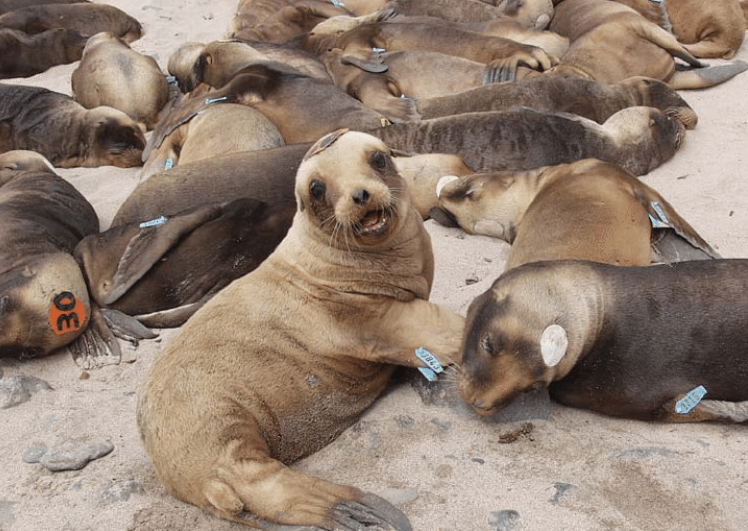
\includegraphics[width=0.6\textwidth]{obrazky-figures/flipperTag.png}
  	\caption{Mláďata lachtanů označená modrými známkami na ploutvích~\cite{NewZeland}.}
  	\label{tag}
  \end{figure}
   
  \subsection*{Čipování}
  Čipy se nejčastěji vkládají pod kůži nebo do břišní dutiny. K~jejich čtení je potřeba speciální čtečka. Jedná se o~trvalou metodu označení, v~porovnání s~ostatními je cenově nákladnější. Pro aplikaci i~čtení čipu je nutno zvíře odchytit. Čip nemusí zůstat na místě, kde byl vložen, může se pohybovat po těle a~tím představovat riziko pro vnitřní orgány~\cite{NewZeland}.
  
  \subsection*{Barvení}
  Barvení je dočasný způsob označení. Barva, aplikovaná na kůži nebo srst zvířat (viz obrázek~\ref{barva}), se časem ztrácí vlivem odlupování kůže nebo vypadávání srsti. Trvanlivost značek závisí na prostředí, chování zvířete a~vlastnostech barvy. Samotné barvení obvykle zvířeti neublíží, ale může zvýšit viditelnost daných zvířat pro lidské pozorovatele i~pro predátory nebo kořist. Také může způsobit, že označená zvířata budou odlišně vnímána svým druhem~\cite{NewZeland}.
  
  \begin{figure}[hbt]
  	\centering
  	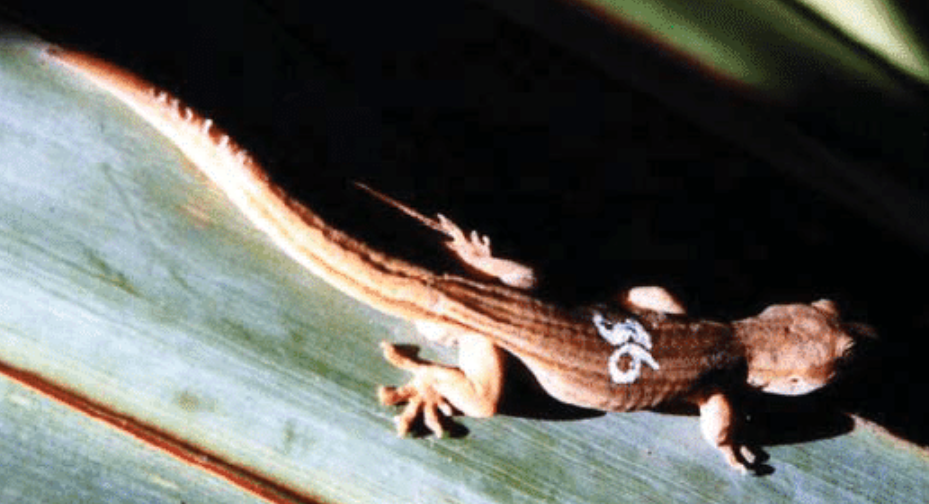
\includegraphics[width=0.7\textwidth]{obrazky-figures/barva.png}
  	\caption{Gekon s~dočasným označením barvou~\cite{NewZeland}.}
  	\label{barva}
  \end{figure}
   
  \subsection*{Označení mrazem}
  Označení mrazem selektivně ničí buňky produkující pigment ve folikulech chlupů, a~tím dochází k~tvorbě bílých chlupů nebo depigmentaci kůže, která kontrastuje s~původní barvou srsti/kůže. Tento proces způsobuje poškození tkání, následnou bolest, stres a~zvyšuje riziko infekce~\cite{NewZeland}.
  
 \subsection*{Výžeh}
  Výžeh způsobuje trvalou jizvu na kůži zvířete (viz obrázek~\ref{branding}), která je výsledkem popáleniny druhého nebo třetího stupně způsobené horkým železem. Popáleniny jsou doprovázeny okamžitými změnami chování spojenými s~akutní bolestí. Úplné zahojení trvá až 8~týdnů. Tento proces také zvyšuje riziko pracovních úrazů pro pracovníky a~kouř vznikající při spálení zvířecí srsti a~kůže má negativní vliv na jejich zdraví. Dobytek si může spojit člověka s~bolestí a~začít vykazovat vysokou reaktivitu, to negativně ovlivňuje interakci mezi člověkem a~zvířetem~\cite{IronBranding}.
  
  \begin{figure}[hbt]
  	\centering
  	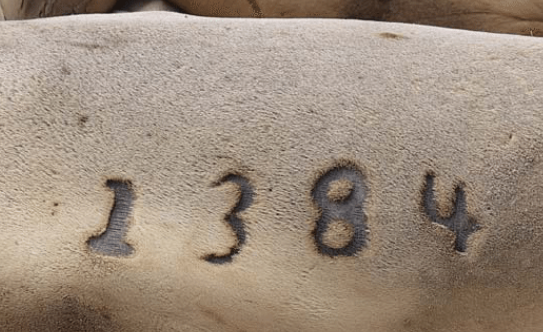
\includegraphics[width=0.55\textwidth]{obrazky-figures/branding.png}
  	\caption{Dospělá samice tuleně označená výžehem~\cite{NewZeland}.}
  	\label{branding}
  \end{figure}
  
  
\subsection*{Tetování}
 Tetování je považováno za trvalou metodu označení zvířat, ale trvanlivost závisí na druhu a~věku zvířete, kvalitě provedení a~umístění značky. Vyžaduje dlouhodobé zadržení zvířete během aplikace, je bolestivé, může způsobit infekci a~zvíře je třeba opět odchytit při čtení tetování. Tetování může také vyblednout nebo se jinak stát nečitelným. Nejlepších výsledků se dosahuje tetováním jakékoli jemně pigmentované oblasti, která je čistá a~relativně bez srsti~\cite{NewZeland}. 
  

\section{Biometrie zvířat}
\label{biometrie}
Biometrické technologie, jako je rozpoznávání otisků prstů, obličeje, duhovky či cév, jsou dnes běžně používány pro identifikaci lidí. Díky jejich úspěšnosti nacházejí uplatnění i~při identifikaci zvířat~\cite{beagle}. Na rozdíl od tradičních metod biometrická identifikace nezpůsobuje zvířatům bolest ani nemění jejich vzhled. Biometrické rysy jsou přirozeně jedinečné, nereplikovatelné, opakovaně použitelné, měřitelné a~charakterizované výraznými fyzickými znaky. Ve srovnání s~tradičními metodami biometrické systémy nabízejí vyšší úroveň přesnosti a~spolehlivosti, čímž minimalizují riziko záměny nebo podvodů~\cite{Cihan}. V~kontextu identifikace zvířat se využívají různé biometrické charakteristiky, z~nichž některé budou podrobněji probrány v~následujících částech.

\subsection*{Duhovka}
Rozpoznávání podle duhovky je jednou z~nejspolehlivějších biometrických technologií. Navíc, jako vnitřní (ale přesto externě viditelný) orgán oka, je duhovka dobře chráněná před vnějšími vlivy a~v~průběhu života se nemění, to z~ní dělá vhodný biometrický rys. Ačkoli jsou systémy rozpoznávání duhovky pro lidi dobře vyvinuté a~běžně používané, u~zvířat představují určité výzvy. Duhovky zvířat mají složitý, často eliptický tvar, a~je obtížné je segmentovat a~kódovat běžnými metodami. Kromě toho jsou snímky často nekvalitní kvůli nespolupracujícímu chování zvířat a~proměnlivým podmínkám prostředí, jako je nejednotné osvětlení. Tento přístup je podrobně popsán v~článku \emph{A~New Cow Identification System Based on Iris Analysis and Recognition}~\cite{iris}, kde navržený algoritmus zaměřený na rozpoznávání duhovek krav dosahuje v~režimu identifikace úspěšnosti 98,33~\%. 

\subsection*{Sítnice}
Cévní vzor sítnice (viz obrázek~\ref{sitnice}), nacházející se na zadní straně oka, představuje jedinečný biometrický identifikátor, který zůstává neměnný po celý život. Používá se pro identifikaci jak u~lidí, tak u~zvířat. Ačkoli je její použití u~zvířat méně prozkoumáno než u~lidí, existují studie zaměřené na druhy, jako jsou ovce, skot, kozy a~psi. 

Dosud byla většina studií na toto téma realizována prostřednictvím specializovaných zařízení, která snímají obraz sítnice a~následně pomocí integrovaného softwaru vytvářejí shodu s~databází. Tato zařízení však mají omezené možnosti zpracování obrazu a~aktualizace bývají nákladné. Využití metod zpracování obrazu by mohlo nabídnout větší flexibilitu, přizpůsobitelnost a~potenciálně pokrýt širší spektrum zvířecích druhů~\cite{Cihan}.

Článek \emph{CattNIS: Novel Identification System of Cattle with Retinal Images Based on Feature Matching Method}~\cite{CattNIS} popisuje vývoj nového systému pro identifikaci skotu na základě snímků retinálních vzorců. V~rámci vyvinutého systému \texttt{CattNIS} dosáhla metoda \texttt{SURF} nejvyšší úspěšnosti identifikace, a~to 92,25~\%. Výsledky této studie ukazují, že identifikace skotu na základě vzorců cévního systému sítnice je velmi úspěšná.

\begin{figure}[hbt]
	\centering
	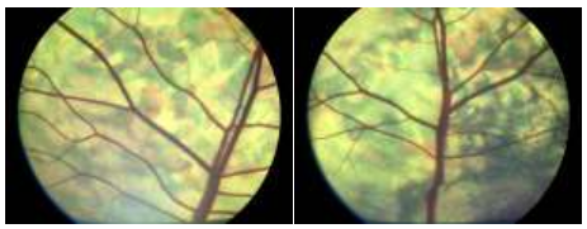
\includegraphics[width=0.7\textwidth]{obrazky-figures/sitnice.png}
	\caption{Identifikace na základě snímků sítnice. Dva příklady snímku sítnice znázorňují cévní struktury, které slouží jako jedinečný biometrický identifikátor~\cite{Cihan}.}
	\label{sitnice}
\end{figure}

\subsection*{Vzory srsti}
Biometrická identifikace zvířat využívá jedinečné vzory na srsti, kůži nebo šupinách, například barevné prstence na hadí kůži, vzory na břiše hus nebo obrazce na křídlech motýlů. Tyto rysy jsou unikátní pro každého jedince a~umožňují provádět pozorování na dálku, čímž se minimalizuje stres a~narušení přirozeného chování zvířat~\cite{Cihan}.

Článek \emph{Biometric Animal Databases from Field Photographs: Identification of Individual Zebra in the Wild}~\cite{zebraID} představuje algoritmus \texttt{StripeCode}, který je jednoduchý na implementaci a~úspěšný při identifikaci zeber z~fotografií pořízených v~terénu. Algoritmus dosahuje dobrých výsledků. Při databázi s~85 jedinci zůstává medián správné pozice pod hodnotou 5.
\texttt{StripeCode} je vhodný pro zvířata s~výraznými vzory srsti či kůže, skládajícími se z~relativně velkých morfologických rysů a~malého počtu barev, například zebry, žirafy nebo tygři. Jeho hlavní omezení spočívá v~tom, že vzhled divokých zvířat není stálý a~může se měnit vlivem zranění, jizev, růstu, stárnutí nebo březosti. Přesto však algoritmus vyniká snadností použití a~schopností pracovat s~fotografiemi pořízenými na dálku, například z~fotopastí, aniž by narušoval život zvířat.
I~přes nižší přesnost ve srovnání s~jinými zmíněnými metodami je \texttt{StripeCode} díky své jednoduchosti a~přístupnosti cenným nástrojem pro biometrickou identifikaci zvířat.

\subsection*{Tvary ploutví}
Systémy pro rozpoznávání založené na tvaru ploutví jsou efektivní metodou identifikace jednotlivých zvířat, zejména u~velryb a~delfínů. Využívají algoritmy pro analýzu okrajů ploutví, které se zaměřují na charakteristické rysy, jako jsou jizvy, zářezy a~tvar ploutví. 

Článek \emph{Flukebook: an open-source AI platform for cetacean photo identification}~\cite{Flukebook} uvádí jako příklad algoritmus \texttt{CurvRank}, který generuje kód kontury na základě digitální analýzy zakřivení okraje ocasní nebo hřbetní ploutve (viz obrázek~\ref{CurvRank}) a~porovnává jej s~databází. Tento algoritmus byl původně aplikován na ocasní ploutve keporkaků, ale postupně byl rozšířen na hřbetní ploutve delfínů a~některé další charakteristické rysy jiných druhů, jako jsou hřbetní hrboly šedých velryb. Při identifikaci podle ocasní ploutve keporkaka má \texttt{CurvRank~v2} úspěšnost 85~\% a~podle hřbetní ploutve delfína skákavého má \texttt{CurvRank~v1} úspěšnost 95~\%. Díky těmto vlastnostem se \texttt{CurvRank} stal významným nástrojem v~oblasti identifikace mořských savců a~přispívá k~jejich ochraně a~výzkumu.

\begin{figure}[hbt]
	\centering
	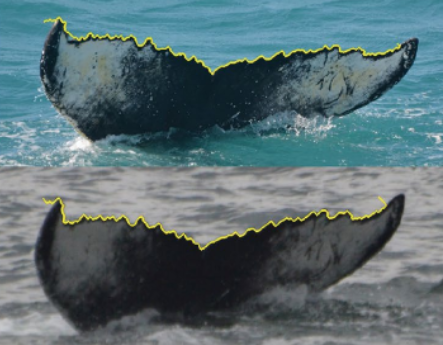
\includegraphics[width=0.5\textwidth]{obrazky-figures/CurvRank.png}
	\caption{Identifikace na základě tvaru ploutví. Shoda nalezená algoritmem \texttt{CurvRank} na základě tvaru ocasní ploutve~\cite{Flukebook}.}
	\label{CurvRank}
\end{figure}


\subsection*{Vzory skvrn v~oblasti vousů}
Článek \emph{Computer-aided photo-identification system with an application to polar bear based on whisker spot patterns}~\cite{polar} popisuje vývoj počítačového systému pro fotoidentifikaci zvířat s~výraznými přírodními rysy, který byl aplikován na lední~medvědy na základě jejich vzorů skvrn v~oblasti vousů, jak je znázorněno na obrázku~\ref{bear}. Tyto skvrny se nacházejí u~základu folikul hmatových vousů a~jsou uspořádány do jedinečného vzoru na každé straně přední části čenichu, což umožňuje spolehlivou identifikaci jednotlivých jedinců. Při vyloučení fotografií nízké kvality a~nevhodného úhlu dosahuje systém pravděpodobnosti správné identifikace přes 80~\% při 10\% pravděpodobnosti falešné identifikace. Jeho výhodou je možnost pořízení fotografie z~dálky bez nutnosti odchytu zvířete, tím minimalizuje stres pro zvířata a~umožňuje neinvazivní sledování. Systém má potenciál být aplikován i~na další druhy s~podobnými charakteristickými vzory, například na lvy, a~mohl by být užitečný při studiu a~ochraně volně žijících a~ohrožených druhů.
\begin{figure*}[h]\centering
	\centering
	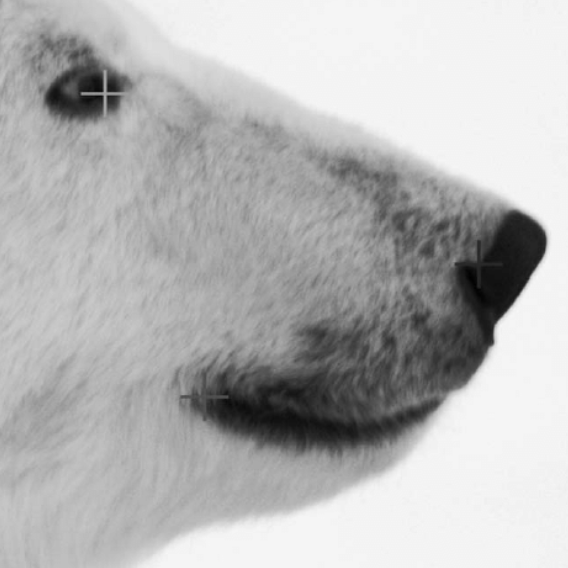
\includegraphics[width=0.4\linewidth]{obrazky-figures/bear.png}
	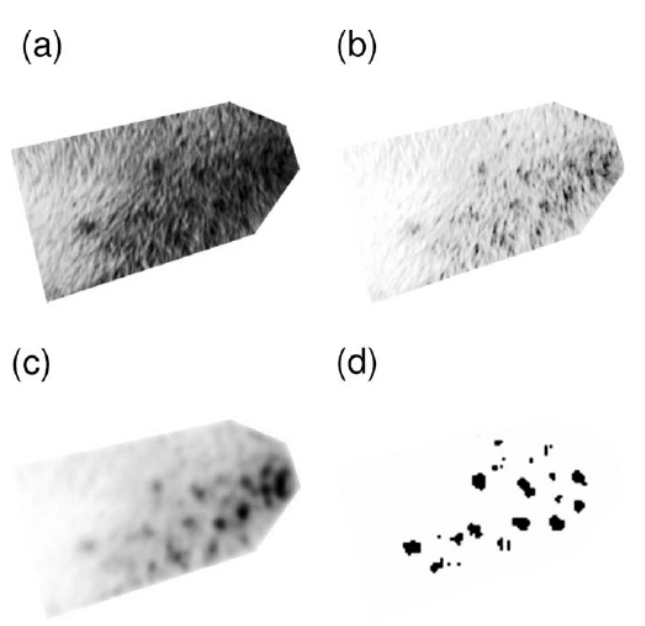
\includegraphics[width=0.4\linewidth]{obrazky-figures/bearProc.png}
	\caption{Vzory skvrn v~oblasti vousů. Levá část obrázku ukazuje vstupní fotografii medvěda, která se použije k~identifikaci. Pravá část (a--d) demonstruje jednotlivé kroky extrakce rysů~\cite{polar}.}
	\label{bear}
\end{figure*}

\section{Biometrická identifikace podle čenichu}
\label{čenich}
Otisky čenichu zvířat vykazují jedinečné charakteristiky, které lze přirovnat k~otiskům prstů u~lidí. Tyto rysy jsou specifické pro každého jedince a~v čase se nemění. Vzhledem k~relativní jednoduchosti jejich získávání oproti jiným biometrickým metodám se staly předmětem intenzivního výzkumu. Významnou roli v~této oblasti sehrávají metody strojového učení. V~posledních letech nabývají na významu zejména techniky hlubokého učení pro ověřování identity a~rozpoznávání jedinců.

Otisky čenichu se s~úspěchem využívají u~různých druhů zvířat, jako jsou psi, krávy nebo koně. Mezi hlavní výhody této metody patří nízké náklady a~minimální invazivita. Sběr dat nevyžaduje přímý zásah do organismu a~nepředstavuje pro zvíře stresující situaci. Přesto však mohou výsledky ovlivnit vnější podmínky, například znečištění, vlhkost nebo nevhodné světelné poměry, které snižují kvalitu pořízených snímků. Další výzvou může být sběr dat od velkých či nebezpečných zvířat a~také rozdíly mezi snímky pořízenými různými typy kamer, které mohou ztížit jejich porovnávání~\cite{kafkas}.

\subsection*{Struktura čenichu} 
Povrch čenichu zvířete tvoří složitý a~nezaměnitelný vzor, který se skládá ze dvou základních prvků -- tzv.~políček a~brázd. Políčka připomínají ostrovy, zatímco brázdy je obklopují ve formě prohlubní podobných tokům řek, jak je vidět na obrázku~\ref{structure}. Tato struktura je srovnatelná s~otisky prstů u~lidí. Každý jedinec má specifické uspořádání těchto prvků, které se liší nejen tvarem a~rozmístěním, ale také barevným vzorem. Zbarvení čenichu bývá částečně charakteristické pro jednotlivá plemena, ale u~každého zvířete se vyskytují jemné odchylky, které mohou sloužit jako doplňující rozlišovací znak. Kombinace těchto strukturálních a~barevných rysů umožňuje nejen určování plemene, ale i~identifikaci konkrétního jedince~\cite{Kumar}.

\begin{figure}[hbt]
	\centering
	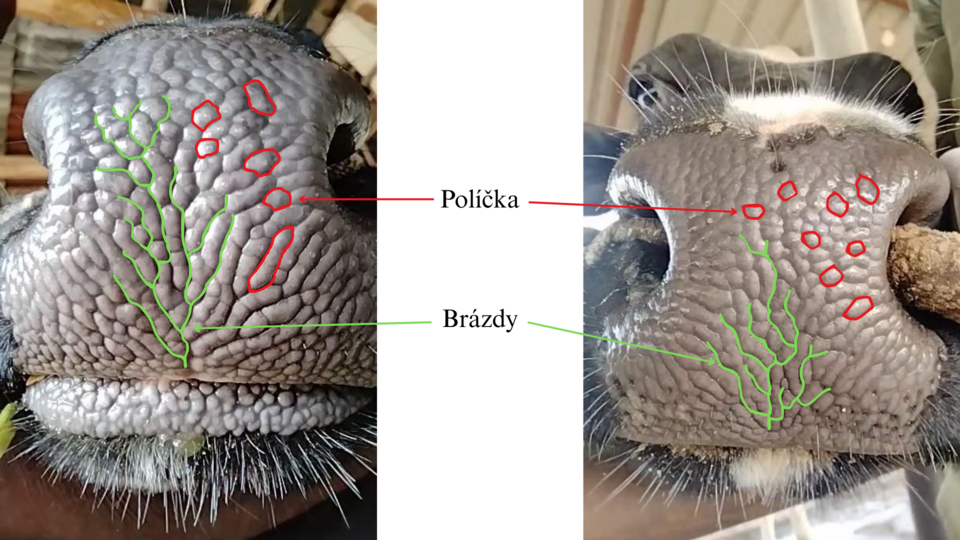
\includegraphics[width=0.8\textwidth]{obrazky-figures/structure.png}
	\caption{Struktura čenichu skotu s~vyznačením základních identifikačních rysů -- políček (červeně) a~brázd (zeleně). Původní fotografie převzaty z~datasetu~\cite{dvc-5_dataset}.}
	\label{structure}
\end{figure}

\subsection*{Ověření jedinečnosti}
V článku \emph{The Formation and Invariance of Canine Nose Pattern of Beagle Dogs from Early Puppy to Young Adult Periods} \cite{beagle} se autoři zaměřili na ověření, zda je vzor čenichu psa řádně formován již v~nejranější navrhované době pro adopci a~zda tento vzor zůstává neměnný během růstu štěněte až do období mladé dospělosti. 
I~když existuje mnoho studií, které potvrzují jedinečnost vzoru čenichu u~psů a~jiných zvířat, všechny dosavadní výzkumy byly založeny na vzorcích shromážděných v~krátkém časovém období, aniž by byly provedeny následné studie na delší časové škále. 

Dalším významným aspektem článku je zaměření na sourozence. Pokud by otisky čenichu nebyly jedinečné, dalo by se očekávat, že podobnosti se nejčastěji projeví mezi geneticky podobnými jedinci. Studie se proto zaměřila na sourozence ze dvou vrhů stejného plemene (beagle) od dvou různých matek a~každý měsíc pořizovala snímky od 2. do 11. měsíce života. 

Výsledky ukazují, že při srovnávání dvou obrázků stejného psa byla maximální vzdálenost shody 0,3577, zatímco u~obrázků různých psů byla minimální vzdálenost 0,4254. To znamená, že vzor čenichu stejného psa je vždy odlišný od vzoru čenichu psa jiného. Pro rozhodování o~shodě byl použit práh 0,4: pokud je vzdálenost shody menší než tento práh, obrázky pocházejí od stejného psa, pokud je větší, pak od různých psů. Tento proces rozhodování neprodukuje žádné chyby. To prokazuje, že vzor čenichu psa ve věku dvou měsíců zůstává stejný po celý jeho život (viz obrázek~\ref{beagle}). Na druhé straně vzory čenichu různých psů jsou vždy odlišné, bez ohledu na to, kdy byly obrázky pořízeny. Vzor čenichu je spolehlivý biometrický rys.

\begin{figure}[hbt]
	\centering
	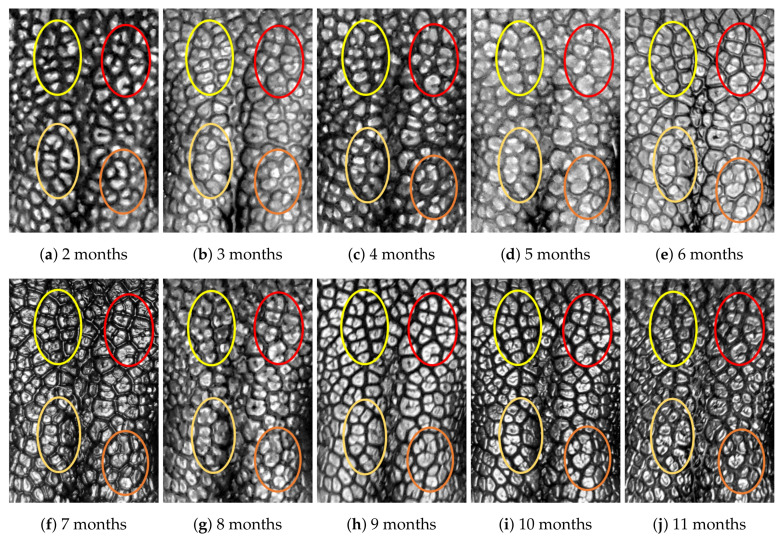
\includegraphics[width=0.9\textwidth]{obrazky-figures/beagle.jpg}
	\caption{Snímky čenichu stejného jedince od 2. do 11. měsíce života. Barveně jsou znázorněny shodné struktury políček a~brázd~\cite{beagle}.}
	\label{beagle}
\end{figure}

\subsection*{Existující řešení}
Otisky čenichů zvířat byly studovány již dlouhou dobu, výzkumy sahají až do počátku 20.~let 20.~století. První studie zahrnovaly zpracování inkoustových otisků, inkoust byl nanesen na čenich zvířete a~následně přenesen na papír, jak lze vidět na obrázku~\ref{nosePrint}. V~roce 1922 W.~Petersen studoval otisky čenichu více než 350~krav a~dospěl k~závěru, že žádná dvě zvířata nemají identický vzor a~že otisky čenichů poskytují spolehlivý způsob identifikace. Později však bylo uznáno, že otiskování je dlouhý a~náročný proces, který způsoboval stres zvířatům. Navíc otisky nebyly dostatečně kvalitní pro použití v~počítačovém prostředí~\cite{kafkas, Cihan, beagle}.

\begin{figure}[hbt]
	\centering
	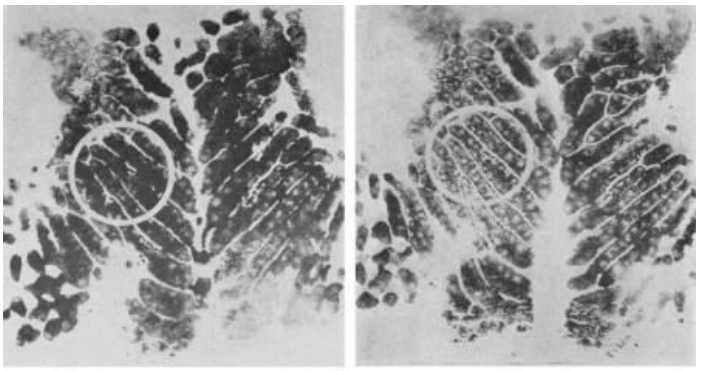
\includegraphics[width=0.6\textwidth]{obrazky-figures/cowID.png}
	\caption{Inkoustové otisky čenichu stejné krávy se znázorněním shodného rysu~\cite{nosePrint}.}
	\label{nosePrint}
\end{figure}

S rozvojem technologií a~metod strojového učení byla biometrická identifikace na základě čenichů zvířat podstatně vylepšena. Tradiční metody byly postupně nahrazeny novějšími přístupy, které umožňují rychlou a~efektivní identifikaci bez nutnosti přímého kontaktu se zvířetem. Jedním z~pokročilých řešení je metoda zpracování čenichu psů, která využívá hluboké neuronové sítě (\textit{deep neural networks}). Například v~článku \emph{Dog Nose-Print Identification Using Deep Neural Networks}~\cite{dog_nose_print} byla navržena síť nazvaná \texttt{DNNet (Dog Nose Network)}, která je schopná extrahovat rysy pro individuální identifikaci psů. Je založená na konvoluční neuronové síti se strukturou siamské neuronové sítě (\textit{Siamese network}), používá ztrátové funkce \textit{Contrastive loss} a~\textit{ArcFace loss}. Nejlepší výsledky byly dosaženy s~použitím sítě ResNet-152, metoda dosáhla při identifikaci přesnosti 98,972~\%.
Pro vytvoření datasetu bylo shromážděno 2~561 fotografií čenichů od 302~psů. Snímky byly získány v~útulcích pomocí běžných mobilních telefonů. Oblast čenichu byla následně manuálně vyříznuta. Tento přístup je nejen jednodušší a~rychlejší než tradiční inkoustové metody, ale také méně invazivní, což výrazně snižuje stres pro zvířata a~zvyšuje praktičnost celého systému.

Článek \emph{Individual Beef Cattle Identification Using Muzzle Images and Deep Learning Techniques}~\cite{VGG} představuje řešení, které dosáhlo přesnosti identifikace 98,7~\%. Bylo použito 4~923~snímků od 268~krav. Snímky byly pořízeny pomocí digitálního fotoaparátu a~krávy nebyly omezeny. Oblast čenichu byla manuálně vyříznuta. Bylo porovnáno 59~modelů pro klasifikaci obrázků pomocí hlubokého učení, nejlepších výsledků dosahovaly architektury VGG se ztrátovou funkcí \textit{cross-entropy loss}.

Studie \emph{Identification of Individual Hanwoo Cattle by Muzzle Pattern Images through Deep Learning}~\cite{Hanwoo} využívá 9~230~snímků od 336~krav plemene Hanwoo. Fotografie byly pořízeny bez přímého kontaktu se zvířaty pomocí mobilních telefonů. Každý jedinec byl fotografován ve čtyřech různých časech. Oblast čenichu byla automaticky ořezána modelem \texttt{YOLOv8}. Byly testovány různé verze modelu EfficientNet v2 v~kombinaci s~několika optimalizačními algoritmy. Nejlepší validační přesnosti 98,1~\% bylo dosaženo při použití varianty \texttt{small} s~optimalizátorem \texttt{Lion}.

Řešení popsané v~článku \emph{Automated Muzzle Detection and Biometric Identification via Few-Shot Deep Transfer Learning of Mixed Breed Cattle} \cite{Few-Shot} dosáhlo ještě vyšší přesnosti 99,11~\%. Tento přístup využívá algoritmus \texttt{YOLOv3} a~ResNet-50. Dataset obsahuje 2~900~snímků od 300~krav. Fotografie byly pořizovány při omezení každého zvířete v~kleci, kdy jeho hlava byla umístěna do držáku. Fotograf stál přibližně 1--2~metry před zvířetem a~pořizoval snímky z~čelního pohledu pomocí fotoaparátu Canon D800.

\chapter{Detekce objektů v~obraze a~rozpoznávání}
\label{kap3}
Počítačové vidění umožňuje počítačovým systémům extrahovat smysluplné informace z~vizuálních dat, jako jsou obrazy a~videa, a~následně je analyzovat. Mezi základní metody počítačového vidění patří segmentace obrazu, klasifikace obrazu, sledování objektů a~detekce objektů~\cite{Rahaman}.

Tato kapitola se zaměřuje na principy detekce objektů v~obraze. Dále se věnuje konceptu vektorových reprezentací, které slouží k~transformaci vizuálních dat do formátů vhodných pro analýzu a~klasifikaci pomocí algoritmů.

\section{Metody detekce objektů}
\label{detekce}
Detekce objektů je oblast počítačového vidění, která se zaměřuje na lokalizaci a~rozpoznávání jednotlivých objektů v~digitálních obrazech a~videích. Tento proces zahrnuje nejen identifikaci konkrétních instancí objektů patřících do předem definovaných kategorií, ale také jejich přesné umístění v~obraze, které je reprezentováno ohraničujícími rámečky.

Úspěšná detekce objektů má zásadní význam pro širokou škálu odvětví, jako je bezpečnost, doprava, medicína a~armáda. Přesto však tato oblast čelí významným výzvám kvůli tzv.~sémantické propasti mezi tím, jak lidé vnímají obrazy a~jak je reprezentují počítače. Lidé vidí obrazy v~kontextu, rozpoznávají barvy, tvary a~vztahy mezi objekty, zatímco počítače reprezentují obrazy jako matice čísel. To vede k~problémům, jako jsou rozdíly v~rámci třídy, změny osvětlení, změny pohledu apod.~\cite{Rahaman}.

Detekce objektů hraje podstatnou roli v~procesu identifikace zvířat podle čenichu, protože umožňuje přesnou lokalizaci čenichu v~obraze a~jeho oddělení od okolního pozadí. Tím získáme oblast zájmu pro následnou biometrickou analýzu, která zajišťuje identifikaci jednotlivých jedinců. Úspěšná detekce zvyšuje přesnost a~spolehlivost celého systému, protože kvalita identifikace přímo závisí na tom, jak přesně je čenich zvířete detekován. Na obrázku~\ref{yoloCow} je ukázán příklad detekce čenichu pomocí algoritmu \texttt{YOLO}, který bude podrobněji popsán v~následujícím textu.

\begin{figure}[hbt]\centering
	\centering
	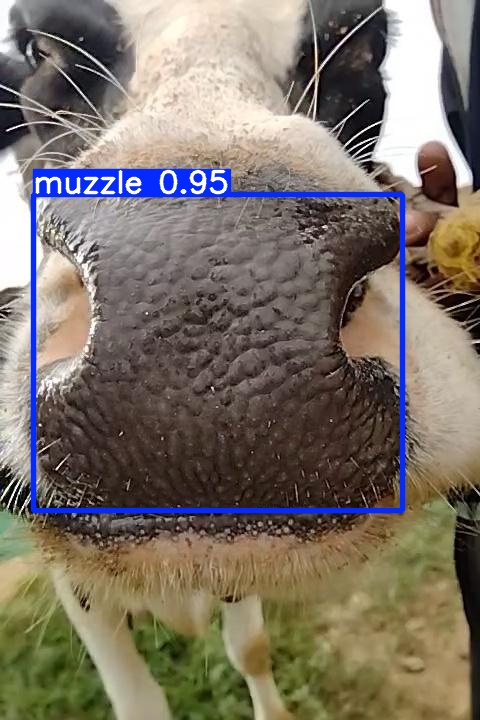
\includegraphics[width=\linewidth, height=6cm, keepaspectratio]{obrazky-figures/yoloCow1.jpg}
	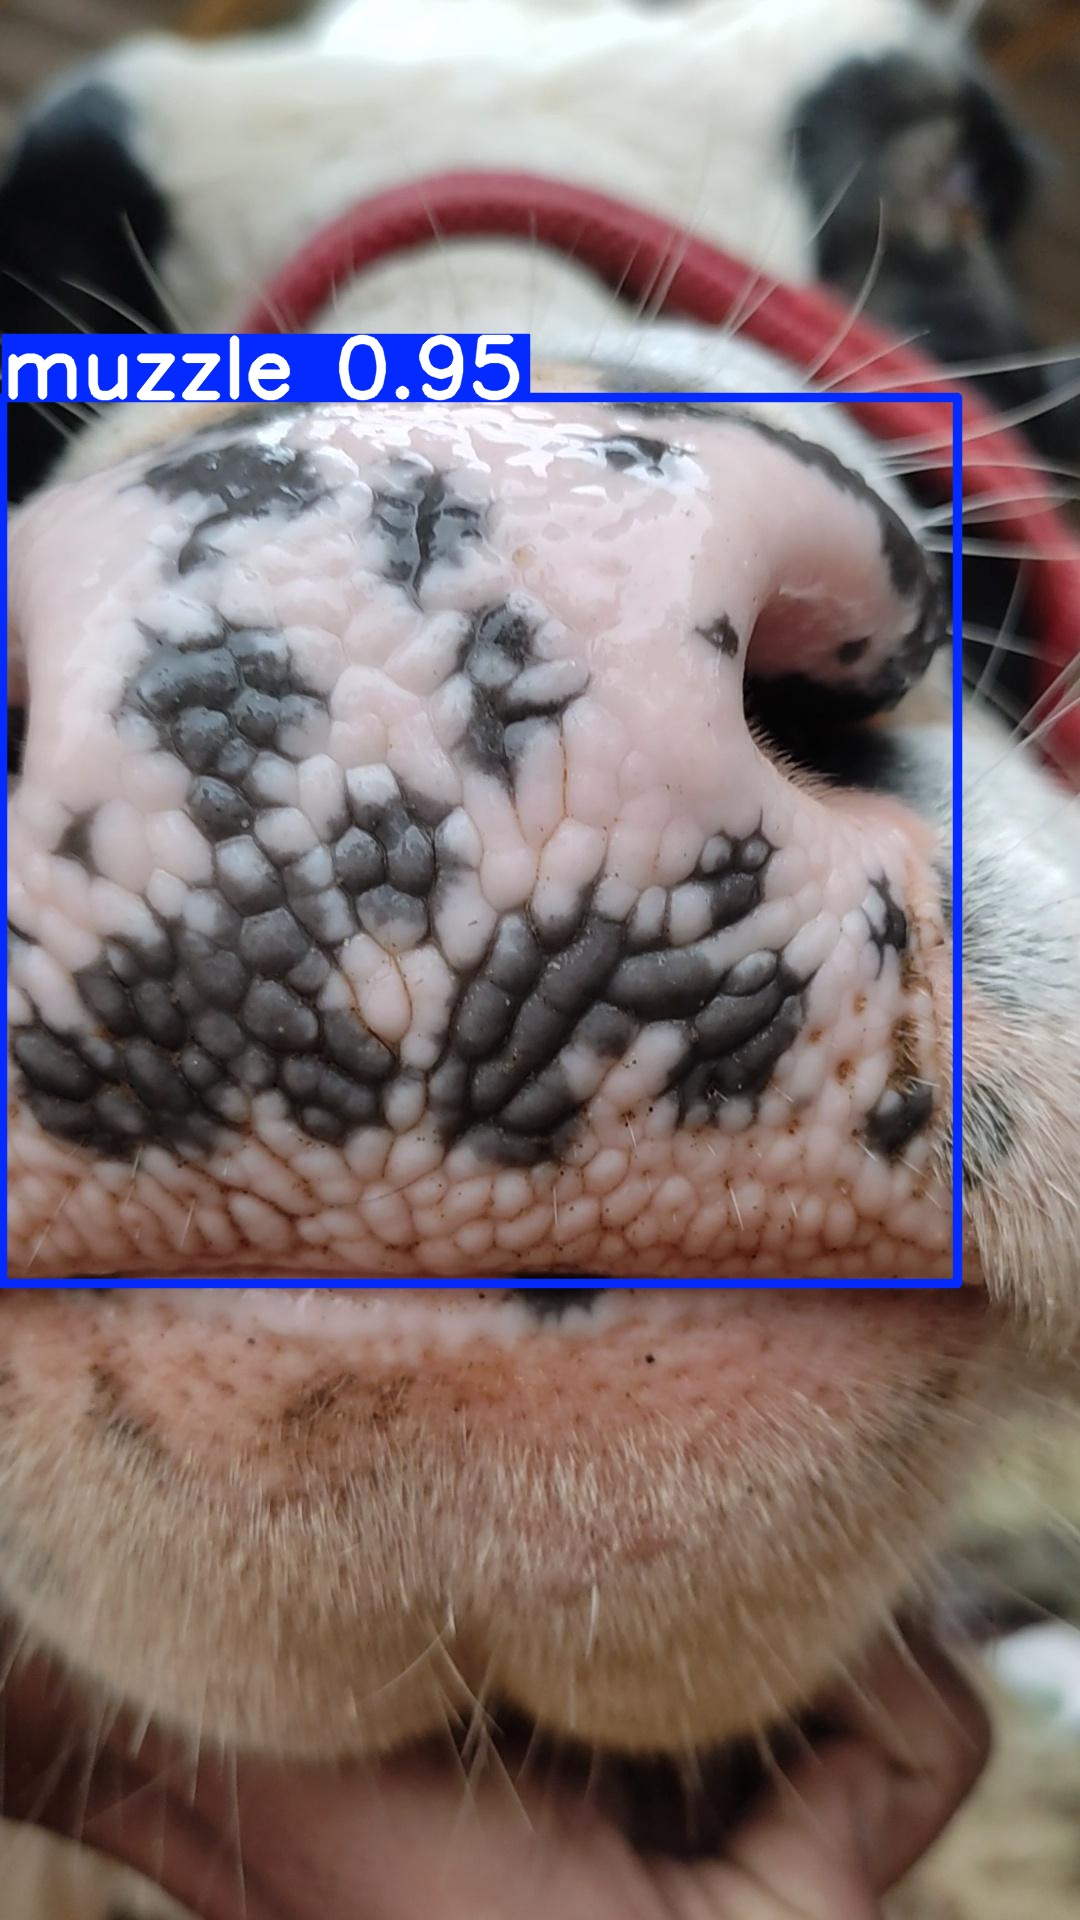
\includegraphics[width=\linewidth, height=6cm, keepaspectratio]{obrazky-figures/yoloCow2.jpg}
	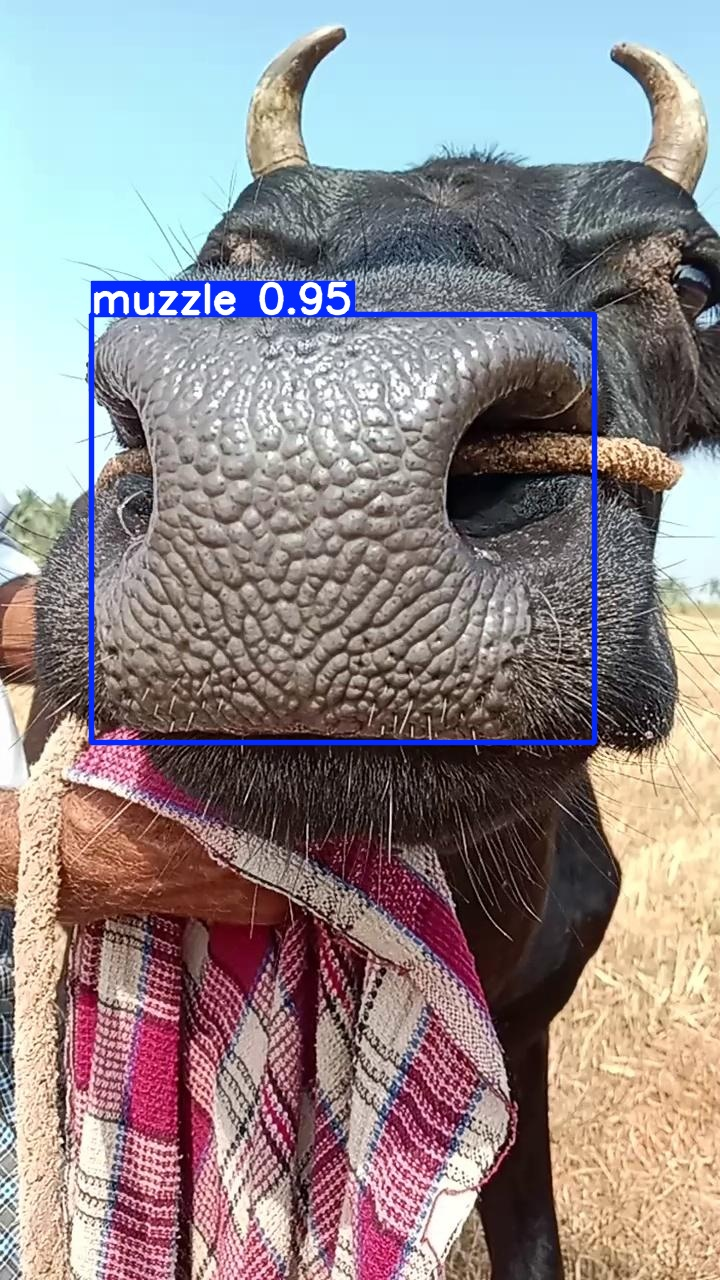
\includegraphics[width=\linewidth, height=6cm, keepaspectratio]{obrazky-figures/yoloCow3.jpg}
	\caption{Příklady uspěšné detekce čenichu krávy pomocí algoritmu YOLO. Původní fotografie převzaty z~datasetu~\cite{dvc-5_dataset}.}
	\label{yoloCow}
\end{figure}


Detektory založené na konvolučních neuronových sítích lze rozdělit na jednostupňové a~dvoustupňové. Dvoustupňové detektory nejprve navrhnou potenciální oblasti zájmu, kde bude provedena klasifikace, a~následně ve druhé fázi provedou samotnou klasifikaci a~lokalizaci. Naproti tomu jednostupňové detektory nepoužívají návrh oblastí, ale považují všechny části obrazu za potenciální objekty a~provádějí klasifikaci a~lokalizaci v~jediném kroku~\cite{Rahaman, Alhardi}.

Dvoustupňové detektory zahrnují \texttt{R-CNN}, \texttt{Fast R-CNN}, \texttt{Faster R-CNN} a~\texttt{Mask R-CNN}. \texttt{R-CNN (Region-Based Convolutional Neural Network)} byl první z~této skupiny, použil selektivní hledání k~identifikaci potenciálních oblastí zájmu, které byly následně klasifikovány pomocí konvolunční neuronové sítě (CNN). \texttt{Fast R-CNN} zrychlil proces tím, že příznaky byly extrahovány pouze jednou pro celý obraz. \texttt{Faster R-CNN} následně integroval \texttt{Region Proposal Network} (\texttt{RPN}) přímo do architektury CNN a~tím zrychlil generování oblastí zájmu a~celý proces detekce. \texttt{Mask R-CNN} přidal schopnost segmentace objektů na úrovni pixelů. Tento model vytváří masky pro každý objekt, čímž umožňuje přesnější určení tvaru objektů v~obraze. Dvoustupňové detektory poskytují vysokou přesnost, ale jejich nevýhodou je nižší rychlost.
Jednostupňové detektory jsou výrazně rychlejší a~ideální pro aplikace, které vyžadují detekci objektů v~reálném čase~\cite{Rahaman, Alhardi}. V~následujících částech budou podrobněji rozebrány.

\subsection*{Single Shot MultiBox Detector}
\texttt{Single Shot MultiBox Detector (SSD)}~\cite{20years} se stal jedním z~prvních úspěšných jedno\-stupňových detektorů. Hlavní inovací oproti předchozím metodám je schopnost detekovat objekty různých měřítek na různých vrstvách sítě, zatímco starší modely prováděly detekci pouze na vrchních vrstvách. To mu umožňuje dosahovat vysoké přesnosti i~rychlosti.

V~době svého vzniku \texttt{SSD} překonal jak nejrychlejší, tak nejpřesnější detektory: dosáhl rychlosti 59~FPS a~mAP 74,3~\% na testovací sadě VOC2007, což je výrazně lepší než \texttt{Faster R-CNN} (7~FPS, mAP 73,2~\%) a~\texttt{YOLO} (45~FPS, mAP 63,4~\%)~\cite{SSD}.

\subsection*{You Only Look Once}
\label{yolo}
\texttt{You Only Look Once (YOLO)}~\cite{20years}, v~překladu \uv{Podíváš se jen jednou}, je první jednostupňový detektor objektů, který analyzuje celý obraz najednou místo generování návrhů regionů. Využívá jednu neuronovou síť, která rozdělí vstupní obraz na mřížku; každá buňka této mřížky pak predikuje ohraničující boxy a~jejich pravděpodobnosti příslušnosti k~jednotlivým třídám.

Tento přístup, představený J.~Redmonem a~jeho týmem na konferenci CVPR~2016, znamenal zásadní průlom v~oblasti detekce objektů. Díky kombinaci vysoké rychlosti a~přesnosti se algoritmus rychle zařadil mezi nejvýznamnější detekční metody. Od svého vzniku prochází architektura neustálým vývojem, každá verze přináší vylepšení v~oblasti přesnosti, rychlosti nebo efektivity~\cite{Terven, YOLO2024}.
Tato sekce se zaměřuje na funkčnost, architekturu a~jednotlivé verze \texttt{YOLO}, jejich vývoj a~vylepšení, která přinesly.


\subsubsection*{YOLOv1}
\texttt{YOLOv1}~\cite{Terven} sjednotilo proces detekce objektů tím, že detekuje všechny ohraničující boxy současně. Model rozdělí vstupní obrázek na mřížku \(S \times S\) a~pro každou buňku mřížky předpovídá \(B\)~ohraničujících boxů s~pravděpodobností \(C\)~tříd. Každý box obsahuje hodnoty: \(P_c\) (\textit{confidence score}, vyjadřující jistotu modelu, že box obsahuje objekt), \(b_x, b_y\) (souřadnice středu boxu), \(b_h, b_w\) (výška a~šířka boxu). Výstupem je tenzor o~rozměrech \(S \times S \times (B \times 5 + C)\), duplicity jsou odstraněny metodou \textit{non-maximum suppression} (\textit{NMS}). Obrázek~\ref{yoloOut} ukazuje zjednodušený výstupní vektor s~ohledem na mřížku \(3 \times 3\), tři třídy a~jednu třídu na buňku mřížky, což představuje osm hodnot. V~tomto zjednodušeném případě by výstup \texttt{YOLO} byl \(3 \times 3 \times 8\). Obrázek~\ref{nms} znázorňuje typický výstup modelu pro detekci objektů obsahujícího více překrývajících se ohraničujících boxů a~výstup po použití \textit{NMS}.

\begin{figure}[hbt]
	\centering
	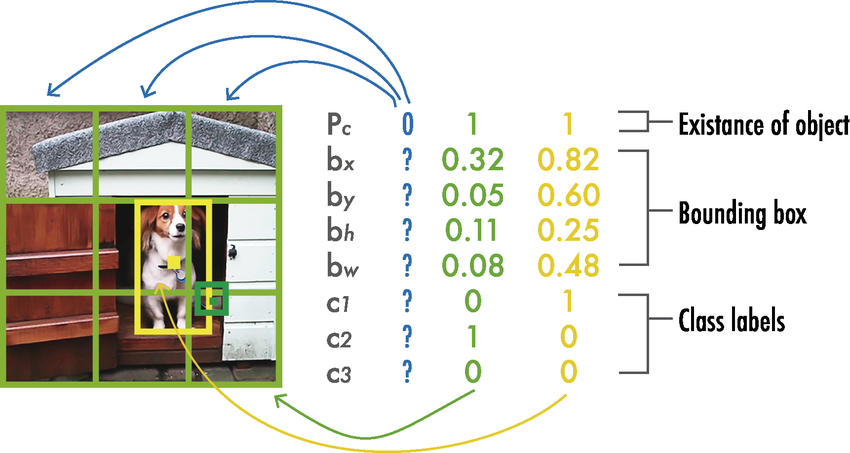
\includegraphics[width=0.7\textwidth]{obrazky-figures/yoloOut.png}
	\caption{\texttt{YOLO} výstupní predikce. Obrázek znázorňuje zjednodušený model \texttt{YOLO} s~mřížkou \(3 \times 3\), třemi třídami a~jedinou predikcí třídy na prvek mřížky pro vytvoření vektoru osmi hodnot~\cite{Terven}.}
	\label{yoloOut}
\end{figure}

\begin{figure}[hbt]
	\centering
	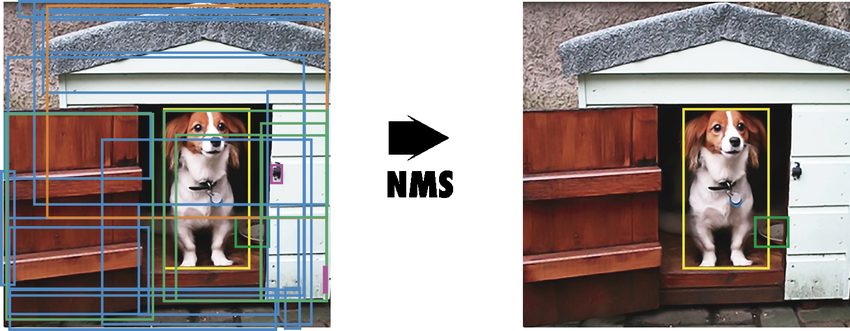
\includegraphics[width=0.7\textwidth]{obrazky-figures/nms.png}
	\caption{\textit{Non-maximum suppression (NMS)}. Vlevo typický výstup modelu detekce objektů obsahující více překrývajících se boxů. Vpravo výstup po \textit{NMS}~\cite{Terven}.}
	\label{nms}
\end{figure}


\texttt{YOLOv1} se skládá z~24~konvolučních vrstev a~2~plně propojených vrstev, které predikují ohraničující boxy a~pravděpodobnosti tříd. Využívá \(1 \times 1\) konvoluční vrstvy inspirované GoogLeNet a~Network in Network pro snížení počtu parametrů a~zlepšení efektivity. Autoři také představili lehčí model nazvaný \texttt{Fast YOLO}, který je složen z~9 konvolučních vrstev.
Model byl předtrénován na datasetu ImageNet při rozlišení \(224 \times 224\) a~následně doladěn pomocí datasetů PASCAL VOC 2007 a~VOC 2012 při rozlišení \(448 \times 448\), což umožnilo přesnější detekci. Pro augmentaci byl použit náhodný posun a~škálování obrazu, stejně jako úpravy expozice a~saturace v~HSV barevném prostoru~\cite{Terven}.

Hlavními faktory ovlivňujícími výkon \texttt{YOLO} byly omezená schopnost detekovat více objektů stejné třídy v~jedné buňce mřížky, potíže s~predikcí objektů s~neobvyklými poměry stran a~omezené učení z~hrubých rysů objektů. Ačkoli \texttt{YOLO} dosahovalo vysoké rychlosti detekce, jeho lokalizační chyby byly větší ve srovnání s~jinými metodami, jako je \texttt{Fast R-CNN}~\cite{Terven}. Výsledky detekce pomocí algoritmu \texttt{YOLOv1} jsou zobrazeny na obrázku~\ref{yolov1}.

\begin{figure}[hbt]
	\centering
	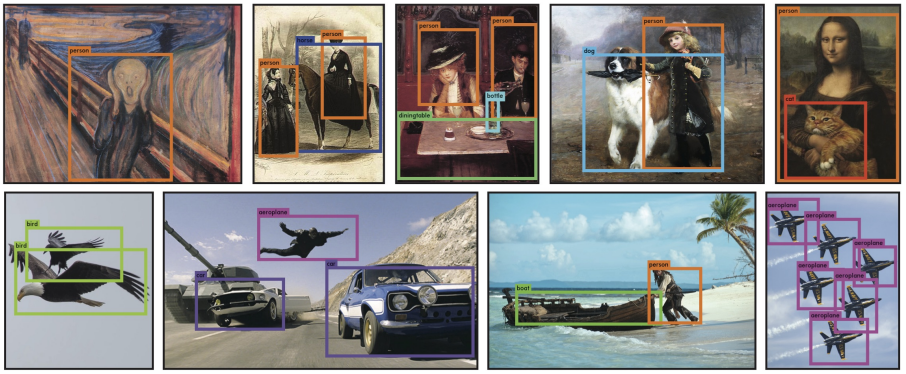
\includegraphics[width=0.9\textwidth]{obrazky-figures/yolov1.png}
	\caption{Ukázka výsledků algoritmu \texttt{YOLOv1}, která správně detekovala všechny objekty kromě jedné osoby, kterou algoritmus označil za letadlo~\cite{yolov1}.}
	\label{yolov1}
\end{figure}

\subsubsection*{YOLOv2}
Nová verze \texttt{YOLOv2}~\cite{Ali2024, Terven} přinesla několik důležitých vylepšení. Využívá síť Darknet19, která obsahuje 19~konvolučních vrstev a~5~\textit{max-pooling} vrstev. Byly odstraněny plně propojené vrstvy a~na každou konvoluční vrstvu byla přidána \textit{Batch Normalization}, která zlepšuje konvergenci modelu a~snižuje riziko přeučení (\textit{overfittingu}). Anchor boxy jsou předdefinované tvary, které síť používá pro predikci ohraničujících boxů objektů v~obraze, jsou znázorněny na obrázku~\ref{yolov2}. Tyto boxy umožňují síti lépe se přizpůsobit objektům různých velikostí a~poměrů stran, čímž zvyšují flexibilitu a~přesnost detekce. Každá buňka mřížky má přiřazeno více anchor boxů, pro které síť predikuje souřadnice a~třídu. Výběr dobrých anchor boxů je důležitý pro dosažení přesných predikcí, provádí se použitím \textit{K-means} klastrování. Tento proces pomáhá najít optimální tvar a~velikost boxů, které odpovídají specifickým objektům v~trénovacích datech, a~zajišťuje lepší vyvážení mezi schopností modelu zachytit objekty a~jeho složitostí.


Dále byl představen \texttt{YOLO9000}~\cite{Liu2020}, schopný detekovat více než 9~000~kategorií objektů v~reálném čase. Toho dosahuje díky společné optimalizační metodě pro simultánní trénování na klasifikačním datasetu ImageNet a~detekčním datasetu COCO s~WordTree pro kombinování dat z~více zdrojů. Tento přístup umožňuje \texttt{YOLO9000} provádět slabě supervidovanou detekci, tedy detekci objektů, které nemají anotace ohraničujících boxů.

\begin{figure}[hbt]
	\centering
	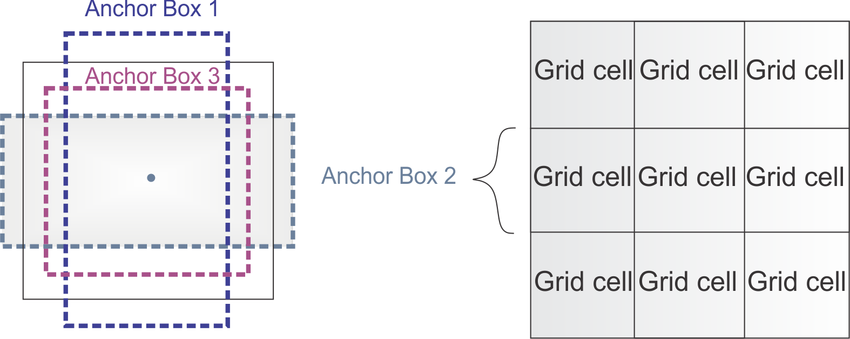
\includegraphics[width=0.7\textwidth]{obrazky-figures/yolov2.png}
	\caption{Anchor boxy. \texttt{YOLOv2} definuje více anchor boxů pro každou buňku mřížky~\cite{Terven}.}
	\label{yolov2}
\end{figure}

\subsubsection*{YOLOv3}
\texttt{YOLOv3}~\cite{Terven, Cong2023} nově využívá síť Darknet-53, která obsahuje 53~konvolučních vrstev s~reziduálními propojeními. Tato hlubší architektura zlepšuje schopnost extrakce charakteristik a~detekční výkon modelu. \texttt{YOLOv3} využívá predikce na více měřítkách (\textit{multi-scale predictions}) a~tím výrazně zlepšuje detekci malých objektů. Využívá tři anchor boxy různých velikostí, které se mohou lépe přizpůsobit objektům různých velikostí a~poměrů stran. Dále byla implementována binární cross-entropie místo softmax funkce, což umožňuje přiřazení více tříd ke stejnému objektu. Tento přístup je užitečný u~datasetů s~překrývajícími se štítky (např. \uv{Člověk} a~\uv{Muž}).

\subsubsection*{Architektura}
V~této době se architektura začala popisovat pomocí tří částí: \textit{backbone}, \textit{neck} a~\textit{head}~\cite{Ali2024, Terven}. 
\begin{itemize}
	\item \textbf{Backbone}: Zodpovídá za extrakci charakteristik ze vstupních dat. Obvykle jde o~konvoluční neuronovou síť předtrénovanou na velkých datasetech, jako je ImageNet. Ve variantách \texttt{YOLO} se jako backbone využívají například ResNet50, ResNet101 nebo CSPDarkNet53.
	\item \textbf{Neck}: Propojuje \textit{backbone} s~\textit{head} a~dále zpracovává a~vylepšuje charakteristiky získané z~\textit{backbone}. Často se využívají techniky, jako jsou \textit{Feature Pyramid Networks (FPN)} nebo \textit{Spatial Attention Modules (SAM)}, které zlepšují reprezentaci rysů a~podporují detekci na různých měřítkách.
	\item \textbf{Head}: Zodpovídá za generování predikcí na základě charakteristik poskytnutých \textit{backbone} a~\textit{neck}. Obvykle obsahuje jednu nebo více podsítí zaměřených na specifické úkoly, jako je klasifikace, lokalizace, segmentace instancí nebo odhad pozic. \textit{Head} vytváří predikce pro jednotlivé kandidáty na objekty a~\textit{post-processing}, například \textit{Non-Maximum Suppression (NMS)}, eliminuje překrývající se predikce a~ponechává pouze ty s~nejvyšší jistotou.
\end{itemize}

\subsubsection*{YOLOv4}
\texttt{YOLOv4}~\cite{Terven, Cong2023} používá jako základní síť CSPDarknet53, která snižuje spotřebu výpočetních zdrojů. Bylo přidáno \textit{Spatial Pyramid Pooling (SPP)} a~reziduální propojení, to zrychluje konvoluční proces a~zlepšuje predikční výkon. Dále byla implementována mozaiková augmentace, která umožňuje detekci objektů mimo běžný kontext, a~regularizace pomocí \textit{DropBlock}. \textit{CIoU (Complete Intersection over Union)} je vylepšením standardního \textit{IoU}, jehož princip je znázorněn na obrázku~\ref{iou}. Optimalizace hyperparametrů a~vylepšení \textit{post-processing} přispívají k~větší přesnosti a~robustnosti detekce.
\begin{figure}[hbt]
	\centering
	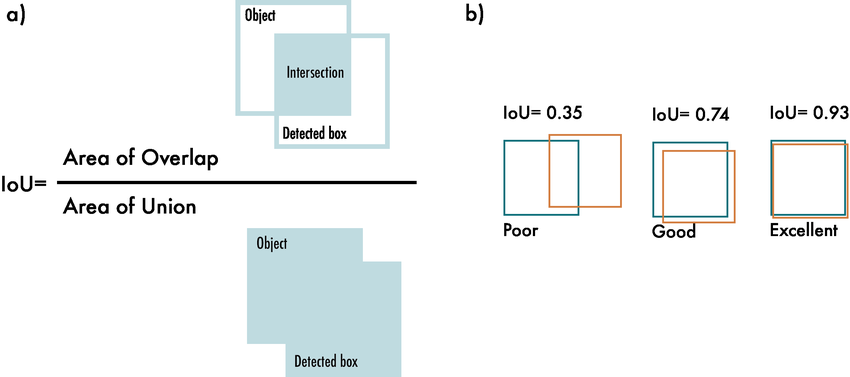
\includegraphics[width=0.9\textwidth]{obrazky-figures/IoU.png}
	\caption{\textit{Intersection over Union (IoU)}. (a)~\textit{IoU} se vypočítá jako podíl průniku dvou rámečků (\textit{boxes}) a~jejich sjednocení; (b)~příklady tří různých hodnot \textit{IoU} pro různá umístění boxů \cite{Terven}.}
	\label{iou}
\end{figure}


\subsubsection*{YOLOv5}
\texttt{YOLOv5}~\cite{Terven} přinesl několik vylepšení oproti předchozím verzím. Přešel z~frameworku Darknet na PyTorch, což zjednodušilo přizpůsobení modelu. Používá vylepšenou verzi CSPDarknet53 s~vrstvou strided konvoluce pro snížení výpočetních nároků a~vrstvou \textit{Spatial Pyramid Pooling Fast (SPPF)} pro optimalizaci využití paměti. \texttt{YOLOv5} implementuje algoritmus \textit{AutoAnchor} pro přizpůsobení anchor boxů pomocí genetického algoritmu, který zlepšuje detekci objektů. Mezi augmentace patří mozaiková augmentace, \textit{copy-paste}, \textit{random affine} a~další z~balíčku \textit{albumentations}. Model je dostupný ve více variantách (\texttt{YOLOv5n} až \texttt{YOLOv5x}), které se liší velikostí a~výkonem, pro různé aplikace a~hardware.

\subsubsection*{YOLOv6}
\texttt{YOLOv6}~\cite{Terven} využívá jako backbone EfficientRep založenou na RepVGG, která zajišťuje vyšší paralelismus a~efektivitu. \textit{Neck} používá \textit{Path Aggregation Network (PAN)} s~bloky \textit{RepBlocks} nebo \textit{CSPStackRep} pro větší modely. Model obsahuje oddělený \textit{head}, který zvyšuje přesnost tím, že odděluje úkoly klasifikace a~regrese. Využívá nový přístup k~přiřazování labelů (\textit{Task alignment learning}) a~nové ztrátové funkce jako \textit{VariFocal loss} pro klasifikaci a~\textit{SIoU/GIoU} pro regresi. Ke zrychlení také vedlo kvantizační schéma použitím \textit{RepOptimizer} a~\textit{Channel-wise distillation}. Bylo představeno osm verzí modelu od \texttt{YOLOv6-N} po \texttt{YOLOv6-L6}.

\subsubsection*{YOLOv7}
\texttt{YOLOv7}~\cite{Terven} využívá \textit{Extended Efficient Layer Aggregation Network (E-ELAN)}, která zlepšuje učení modelu díky efektivnějšímu zpracování gradientů. Zavedena byla nová strategie škálování modelů založených na konkatenaci, při níž se hloubka a~šířka bloků škálují stejným faktorem, tím je zajištěna optimální struktura modelu. Dále implementuje plánovanou re-parametrizaci konvolucí (\textit{RepConvN}) a~využívá pomocný \textit{head} pro usnadnění trénování a~hlavní \textit{head} pro přesné konečné predikce. V~době svého vzniku předčil všechny známé detektory objektů z~hlediska rychlosti a~přesnosti v~rozsahu od 5~FPS do 160~FPS.

\subsubsection*{YOLOv8}
\texttt{YOLOv8}~\cite{Terven} nabízí pět škálovaných verzí a~podporuje různé úlohy počítačového vidění, jako je detekce objektů, segmentace, odhad pozice, sledování a~klasifikace. Model používá \textit{backbone} podobný \texttt{YOLOv5}, s~úpravami vrstvy \textit{CSPLayer}, která je nyní označována jako modul \textit{C2f}. Ten kombinuje vysokoúrovňové rysy s~kontextovými informacemi pro lepší přesnost detekce. Používá oddělený \textit{head}, který zpracovává úlohy detekce objektů, klasifikace a~regrese nezávisle, čímž umožňuje každé větvi soustředit se na specifický úkol a~zvyšuje celkovou přesnost modelu. Model \texttt{YOLOv8-Seg}, zaměřený na sémantickou segmentaci, využívá CSPDarknet53 jako extraktor rysů a~modul \textit{C2f} pro dosažení špičkových výsledků v~detekci objektů i~sémantické segmentaci, při zachování vysoké efektivity.

\subsubsection*{YOLOv9}
\texttt{YOLOv9}~\cite{YOLO2024} využívá princip \textit{Information Bottleneck} a~reverzibilní funkce, které umožňují efektivní zachování podstatných informací a~zlepšují generování gradientů, čímž zajišťují lepší konvergenci a~výkon modelu. Model nabízí pět verzí zaměřených na lehké modely, které minimalizují ztrátu informací během procesu \textit{feedforward}. Mezi významné inovace patří metoda \textit{Programmable Gradient Information (PGI)}, která optimalizuje učení zaměřením na stěžejní gradienty. Dále \texttt{YOLOv9} zahrnuje \textit{GELAN (Gradient Enhanced Lightweight Architecture Network)}, což je nová architektonická inovace zaměřená na zlepšení využití parametrů a~výpočetní efektivity.

\subsubsection*{YOLOv10}
\texttt{YOLOv10}~\cite{YOLO2024} využívá jako \textit{backbone} vylepšenou CSP-Net (\textit{Cross Stage Partial Network}), která zajišťuje efektivnější tok gradientů a~snížení výpočetní redundance. Díky použití \textit{PAN (Path Aggregation Network)} se efektivněji spojují vícerozměrné rysy, to přispívá ke spolehlivější detekcii objektů různých velikostí. Model zavádí \textit{One-to-Many Head}, který během trénování generuje více predikcí pro každý objekt, čímž zvyšuje přesnost učení. Pro proces predikce je použit \textit{One-to-One Head}, který generuje jedinou nejlepší predikci pro objekt, tím eliminuje potřebu \textit{Non-Maximum Suppression (NMS)}, zrychluje \textit{post-processing} a~snižuje latenci. \texttt{YOLOv10} zahrnuje \textit{NMS-FreeTraining}, který používá konzistentní dvojité přiřazení štítků k~redukci latence při inferenci. Dalšími inovacemi jsou využívání velkých konvolučních jader a~částečných \textit{self-attention} modulů, které zlepšují výkon při zachování nízkých výpočetních nákladů. Tato verze nabízí také pět škálovaných verzí, od \texttt{nano} po \texttt{extra-large}. Architektura je zobrazena na obrázku~\ref{yolov10}.

\begin{figure}[hbt]
	\centering
	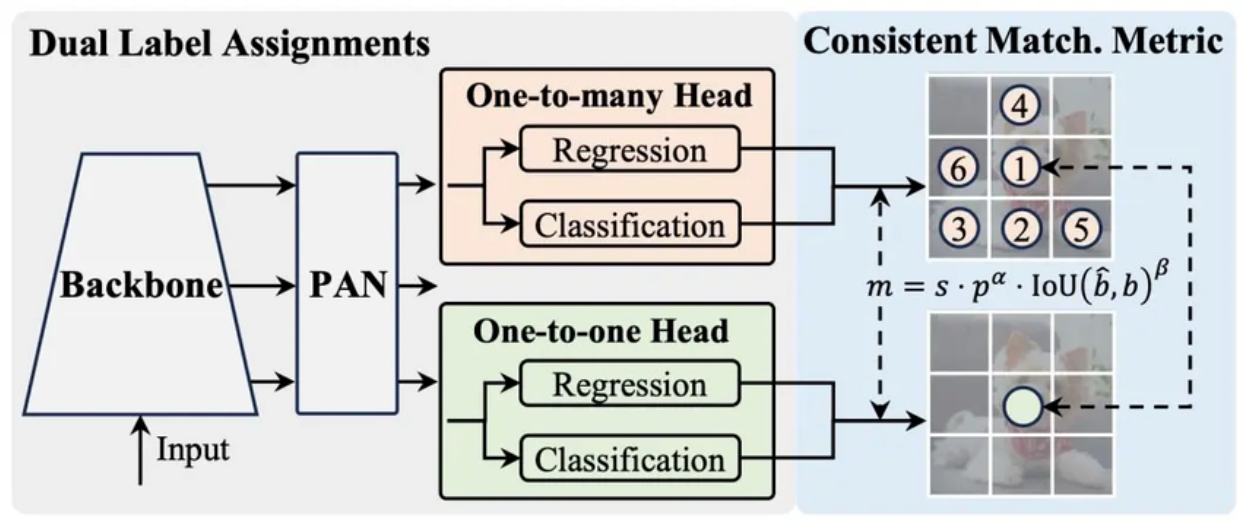
\includegraphics[width=0.85\textwidth]{obrazky-figures/yolov10.png}
	\caption{Architektura \texttt{YOLOv10}, která ukazuje strategii dvojího přiřazování štítků a~vrstvu PAN, \textit{one-to-many head} pro úkoly regrese a~klasifikace a~\textit{one-to-one head} pro přesnou lokalizaci~\cite{YOLO2024}.}
	\label{yolov10}
\end{figure}

\subsubsection*{YOLO11}
\texttt{YOLO11}~\cite{YOLO2024} je nejnovější inovace v~sérii \texttt{YOLO}, která vychází z~vývoje předchozích verzí, zejména \texttt{YOLOv8}. Tato verze nabízí pět škálovaných modelů a~pokrývá různé aplikace. Stejně jako \texttt{YOLOv8} podporuje detekci objektů, segmentaci instancí, klasifikaci, odhad pozice a~detekci orientovaných objektů.
Hlavní novinkou je modul \textit{C2PSA (Cross-Stage Partial with Self-Attention)}, který zlepšuje detekci tím, že efektivněji zachytává kontextové informace napříč vrstvami. Další změnou je nahrazení \textit{C2f} bloku novým \textit{C3k2}, který zvyšuje efektivitu a~rychlost díky menšímu jádru, aniž by to ovlivnilo přesnost. Jak je znázorněno na obrázku~\ref{yolo11}, \texttt{YOLO11} vykazuje lepší výkon než předchozí verze.

\begin{figure}[hbt]
	\centering
	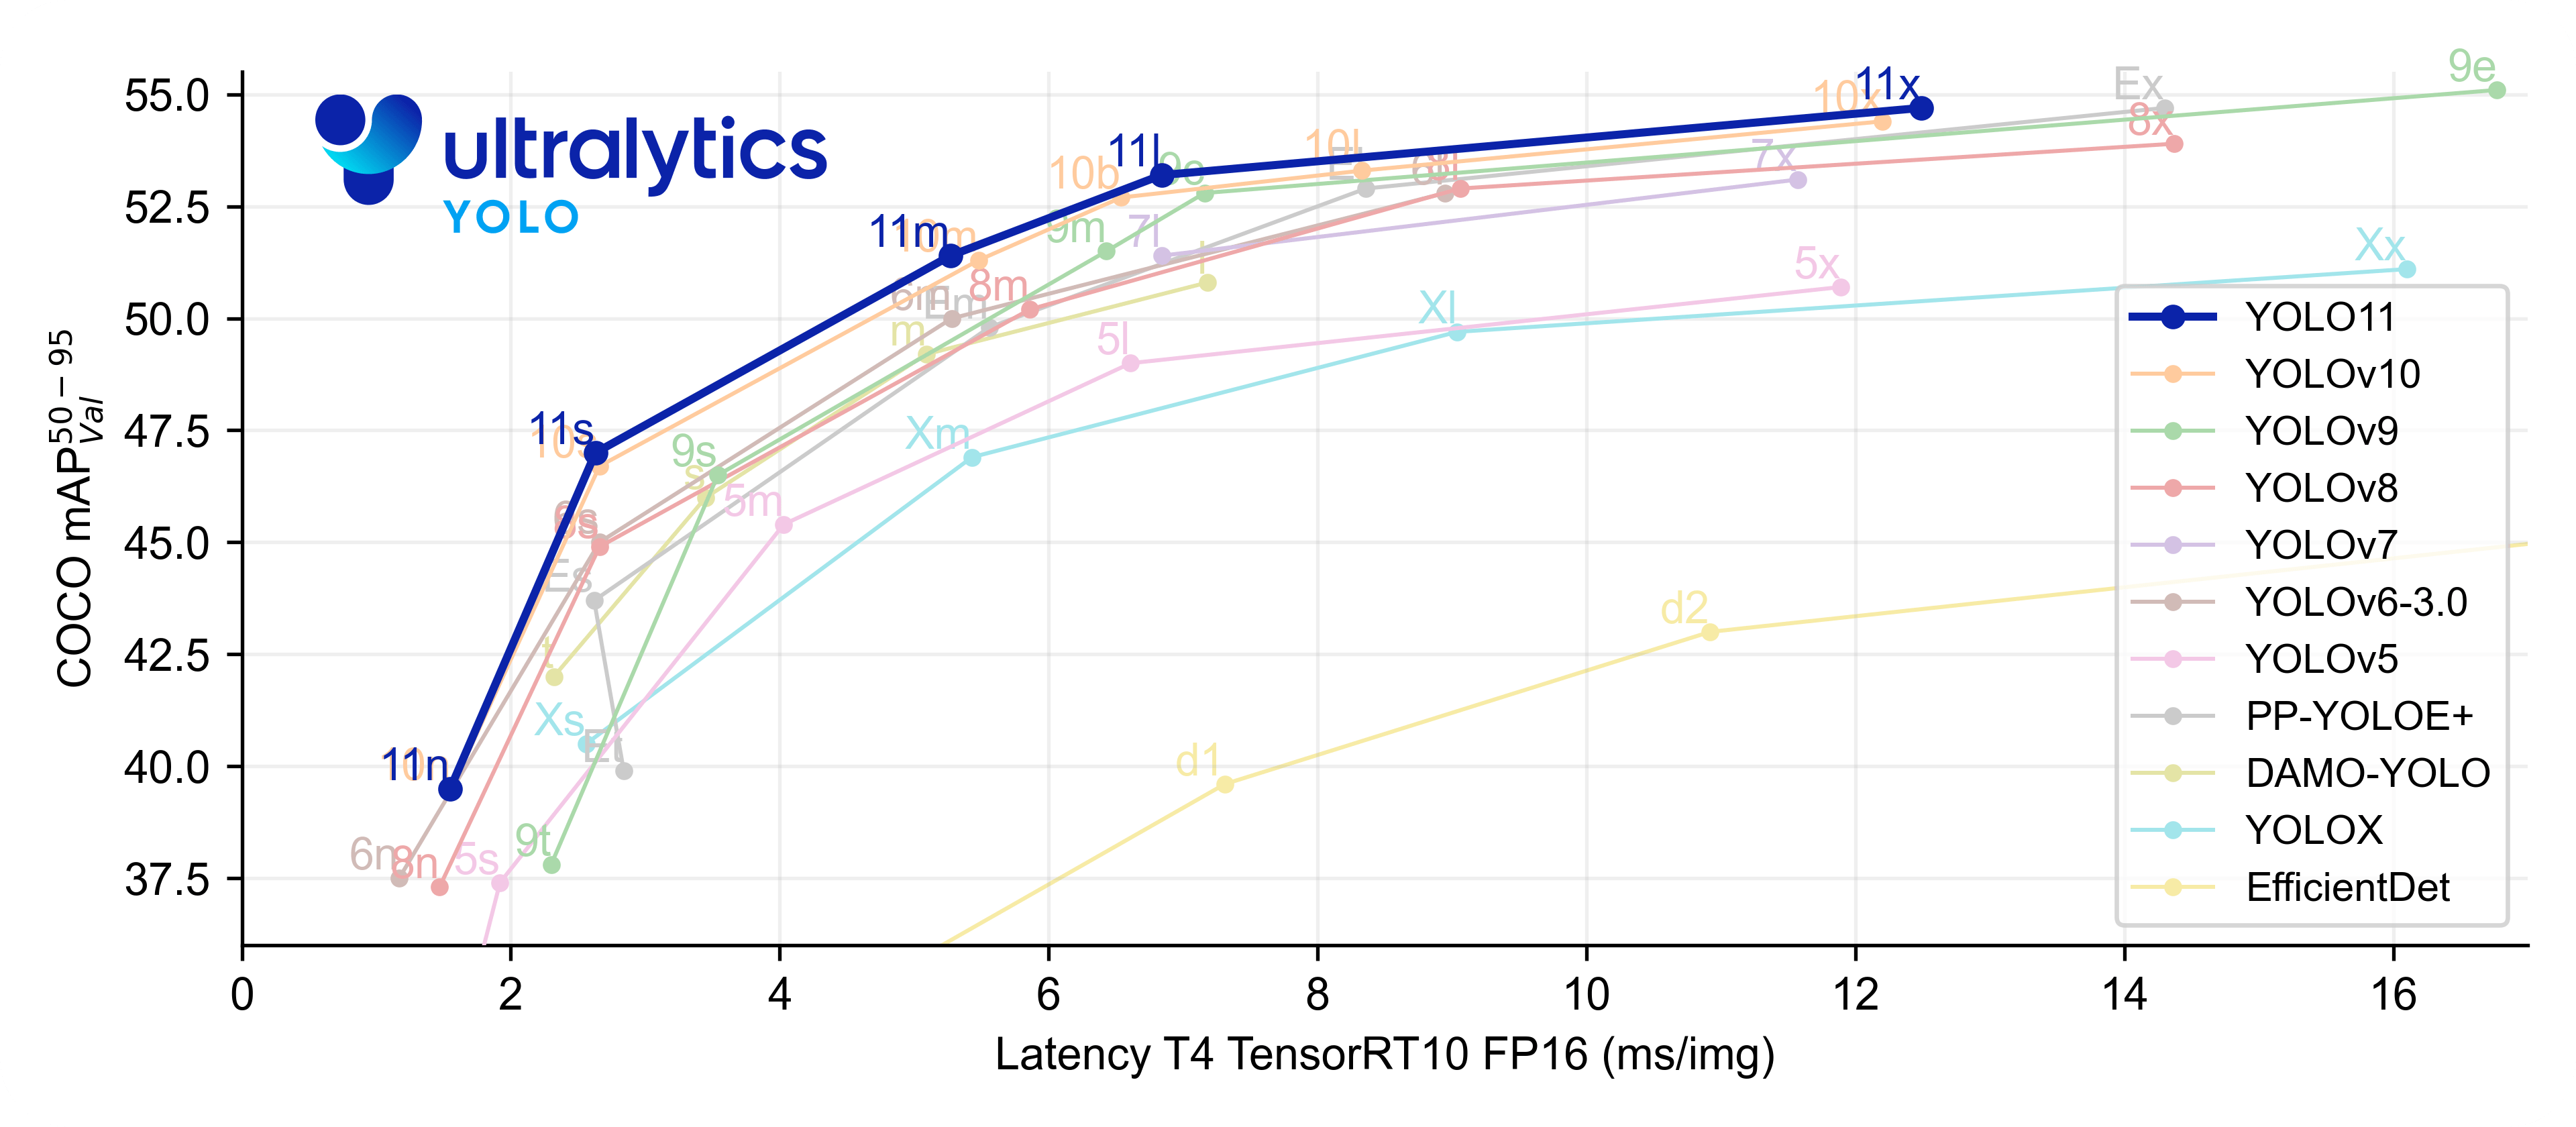
\includegraphics[width=0.95\textwidth]{obrazky-figures/YOLOv11-performance.png}
	\caption{Porovnání výkonu modelu \texttt{YOLO11} s~předchozími verzemi \texttt{YOLO} a~dalšími detekčními modely na datasetu COCO, ukazuje vztah mezi dosaženou přesností a~latencí~\cite{yolo_docs}.}
	\label{yolo11}
\end{figure}

\section{Vektorové reprezentace}
\label{embedding}
K~extrakci vektorových reprezentací obrazových dat se také využívají konvoluční neuronové sítě. Jakmile jsou natrénovány na klasifikaci obrázků, lze jejich konvoluční bloky použít k~extrakci vektorů rysů z~obrazků, který se obvykle nazývá embedding. Konvoluční neuronové sítě se učí klasifikovat obrázky tím, že se učí efektivní reprezentaci vstupu přímo z~nezpracovaných dat; sekvence konvolučních vrstev progresivně zmenšuje velikost vstupních dat a~extrahuje rysy z~obrázků od nízkoúrovňových rysů (např. okraje, intenzity pixelů atd.) v~počátečních konvolučních vrstvách až po vysokoúrovňové sémantické rysy v~posledních konvolučních vrstvách. Poslední konvoluční blok, který je výsledkem trénovacího procesu, je navržen tak, aby generoval vektor s~relevantními rysy~\cite{embedding}.

Tento vektor, tedy embedding, je důležitý pro identifikaci na základě fotografie čenichu. Nejprve je nezbytné detekovat a~vyříznout oblast zájmu (v tomto případě čenich), aby se model soustředil pouze na relevantní vizuální informace. Konvoluční neuronová síť následně extrahuje důležité rysy z~vybrané oblasti a~vrátí embedding. Ten je porovnáván s~ostatními v~databázi. Pokud je vzdálenost mezi embeddingy dostatečně nízká, můžeme prohlásit, že se jedná o~shodu. Vektorová reprezentace tak poskytuje kompaktní a~numericky zpracovatelný formát pro rozpoznávání specifických rysů, které jsou jedinečné pro každého jedince.

\subsection*{Architektury}
Vytváření vektorových reprezentací obrazových dat, známé také jako extrakce příznaků, je zásadním krokem v~analýze dat a~v~mnoha úlohách počítačového vidění. S~příchodem metod hlubokého učení a~zejména konvolučních neuronových sítí došlo k~revoluci v~přesnosti, rychlosti a~množství zpracovávaných dat. Tyto sítě umožňují efektivní zpracování rozsáhlých datových sad a~poskytují data pro další úlohy, včetně klasifikace, detekce objektů nebo segmentace.

Architektury konvolučních neuronových sítí (\textit{backbones}), představují osvědčené modely, které byly původně vyvinuty pro úlohy klasifikace obrázků, ale dnes se používají i~v~dalších oblastech díky jejich schopnosti extrahovat bohaté a~významné příznaky z~obrazových dat. Výběr vhodné architektury závisí na cílovém úkolu a~požadované rovnováze mezi přesností, výpočetní náročností a~rychlostí~\cite{backbones}.
Tyto architektury byly zvoleny na základě jejich osvědčeného výkonu v~úlohách klasifikace a~extrakce rysů, což z~nich činí potenciálně vhodné kandidáty i~pro identifikaci na základě fotografie čenichu.

\subsubsection*{Visual Geometry Group}
Visual Geometry Group (VGG)~\cite{deepCNN} vzniklo s~cílem zjednodušení architektury konvoluční neuronové sítě a~prozkoumání vlivu hloubky sítě na její schopnost reprezentace. ZfNet, která byla přední sítí v~soutěži ILSVRC 2013, naznačila, že použití malých filtrů může zlepšit výkon sítě. Na základě těchto zjištění VGG nahradila filtry o~velikosti \(11 \times 11\) a~\(5 \times 5\) za řadu filtrů \(3 \times 3\). Použití malých filtrů přináší výhodu v~podobě nižší výpočetní složitosti, protože snižuje počet parametrů. Tato zjištění stanovila nový trend ve výzkumu práce s~malými filtry v~konvolučních neuronových sítích. VGG dosahuje vynikajících výsledků v~úlohách klasifikace i~lokalizace obrazů. V~roce 2014 obsadila 2.~místo v~soutěži ILSVRC. Hlavní nevýhodou VGG je použití 138~milionů parametrů, což ji činí výpočetně náročnou a~obtížně použitelnou na systémech s~nízkými prostředky.

\subsubsection*{GoogleNet}
GoogleNet~\cite{deepCNN}, známý také jako Inception-V1, zvítězil v~soutěži ILSVRC 2014 a~jeho hlavním cílem bylo dosáhnout vysoké přesnosti při nízkých výpočetních nákladech. Architektura zavedla inovativní \textit{inception} blok (viz obrázek~\ref{inception}), který využívá více velikostí filtrů (\(1 \times 1\), \(3 \times 3\), \(5 \times 5\)) k~zachycení prostorových informací na různých měřítkách. Tento blok nahrazuje tradiční konvoluční vrstvy a~zvyšuje efektivitu modelu. GoogleNet optimalizuje výpočty přidáním \(1 \times 1\) konvolučních filtrů s~řídkými propojeními, které odstraňují redundantní informace. Použití \textit{global average pooling} vrstvy místo plně propojené vrstvy významně snížilo počet parametrů z~138~milionů na 4~miliony. Model také využívá batch normalizaci, \textit{RmsProp} jako optimalizátor a~pomocné modely pro urychlení konvergence. Hlavními nevýhodami jsou zúžení reprezentace, která může vést ke ztrátě informací, a~heterogenní topologie vyžadující přizpůsobení.
\begin{figure}[hbt]
	\centering
	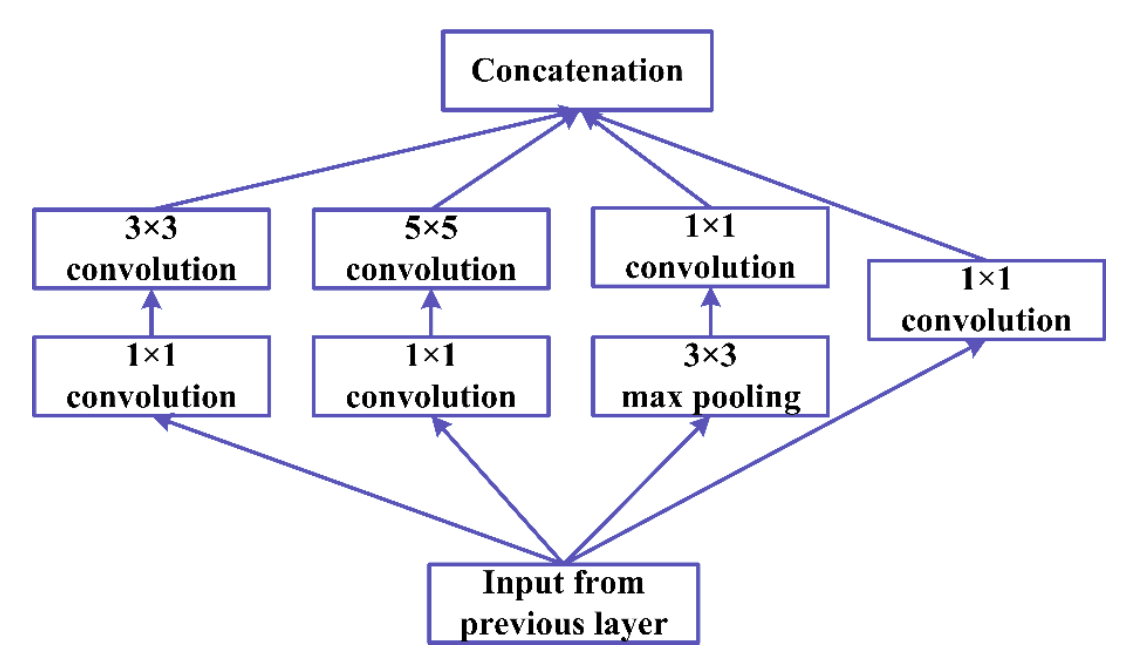
\includegraphics[width=0.7\textwidth]{obrazky-figures/inception.png}
	\caption{Základní struktura \textit{inception} bloku~\cite{deepCNN}.}
	\label{inception}
\end{figure}

\subsubsection*{Residual Neural Network}
Residual Neural Network (ResNet)~\cite{RESNET} byl navržen týmem He Kaiminga z~Microsoft Research Institute. Hlavní motivací pro jeho vznik bylo vyřešení problému degradace neuronových sítí, kdy se při zvětšování hloubky sítě zvyšuje chybovost během trénování. Tento problém je řešen pomocí reziduálních bloků (viz obrázek~\ref{residual}), které umožňují přímý přenos informace mezi vrstvami. Každá vrstva neprovádí přímou transformaci, ale naučí se reziduální funkci (rozdíl mezi požadovaným výstupem a~vstupem), to umožňuje efektivní trénování i~pro velmi hluboké sítě. ResNet zvyšuje svou schopnost extrahovat rysy prostřednictvím propojení rysů mezi vrstvami (\textit{cross-layer feature fusion}), tím umožňuje postupné zlepšování výkonu sítě s~její rostoucí hloubkou. Výzkumný tým otestoval hlubší verze \mbox{ResNet} a~provedl porovnání s~několika jinými modely hlubokého učení. Ukázalo se, že ResNet dosahuje lepších výsledků v~klasifikaci než ostatní modely a~že zvyšováním hloubky lze zlepšit přesnost. 

Verze s~hloubkou 152~vrstev vyhrála soutěž ILSVRC v~roce 2015. ResNet, který byl 20krát a~8krát hlubší než AlexNet a~VGG, vykazoval menší výpočetní složitost. ResNet s~50, 101 nebo 152~vrstvami má nižší chybovost při úloze klasifikace obrazu než 34vrstvá \uv{plain Net} \cite{deepCNN}. 
\begin{figure}[hbt]
	\centering
	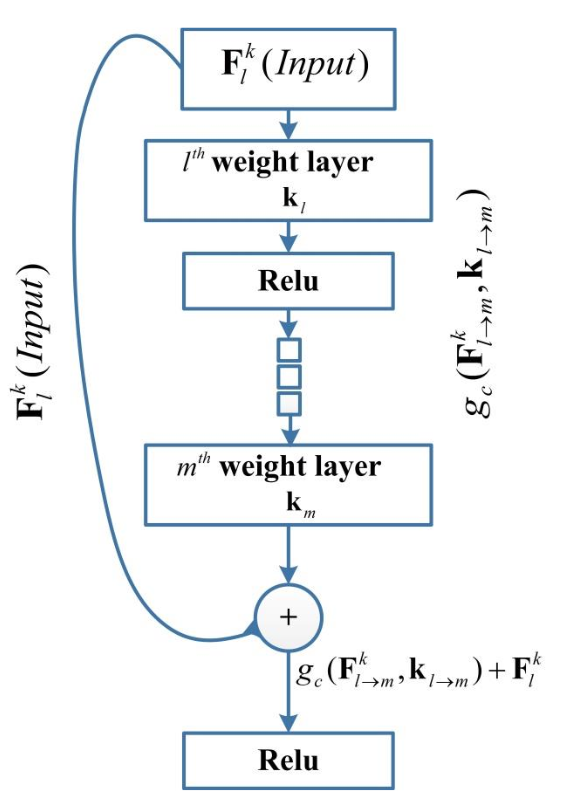
\includegraphics[width=0.4\textwidth]{obrazky-figures/residual.png}
	\caption{Základní struktura reziduálního bloku~\cite{deepCNN}.}
	\label{residual}
\end{figure}

\subsubsection*{MobileNet}
MobileNet~\cite{backbones} je model hlubokého učení vhodný pro zařízení s~nízkým výkonem, jako jsou mobilní zařízení. Architektura MobileNet využívá hloubkově separabilní konvoluce, díky nimž lze model reprezentovat jako odlehčený a~efektivní. Byly zavedeny dva globální hyperparametry, které umožňují vývojářům zvolit vhodnou velikost modelu pro jejich konkrétní problém. MobileNet byl trénován a~testován na ImageNetu pro klasifikaci obrázků.

\subsection*{DenseNet}
DenseNet~\cite{backbones} je konvoluční neuronová síť, která vylepšuje tradiční sítě tím, že každá vrstva využívá výstupy všech předchozích vrstev jako vstupy. Tato architektura má \(L(L + 1)/2\) propojení mezi vrstvami, tím zajišťuje efektivnější tok informací a~umožňuje používat menší výstupní kanály, čímž se snižuje počet parametrů. Počet filtrů v~každé vrstvě se zvyšuje o~konstantu zvanou \uv{míra růstu} (\(k\)), což umožňuje flexibilitu v~počtu parametrů. DenseNet byla navržena v~několika verzích s~různým počtem vrstev (DenseNet-121, DenseNet-169, DenseNet-201 a~DenseNet-264).

\subsubsection*{EfficientNet}
EfficientNet~\cite{backbones} je novější architekturou, která při svém uvedení výrazně překonávala tehdejší modely v~klasifikačních úlohách, a~to i~při menším počtu parametrů a~nižší výpočetní náročnosti. Využívá tzv.~\textit{compound scaling}, tedy jednotné škálování šířky, hloubky a~rozlišení sítě s~cílem dosáhnout co nejefektivnějšího výkonu. Existuje několik verzí EfficientNet, od B0 po B7, konkrétní verzi lze snadno zvolit podle dostupných výpočetních zdrojů. EfficientNet-B0 obsahuje 5,3~milionu parametrů, zatímco poslední verze EfficientNet-B7 má 66~milionů parametrů.

\subsection*{Ztrátové funkce}
Ztrátová funkce je jedním ze základních prvků při trénování neuronové sítě. Udává, jak moc se aktuální výstup modelu liší od správného řešení, a~slouží jako zpětná vazba, podle které se model postupně zlepšuje. Na základě hodnoty ztráty se během trénování upravují váhy neuronové sítě tak, aby se chyba co nejvíce zmenšila.

Hlavním cílem trénování hluboké neuronové sítě je tedy minimalizovat hodnotu ztrátové funkce (čím je menší, tím lépe model rozumí svému úkolu). Výběr vhodné ztrátové funkce závisí na povaze řešené úlohy. Některé funkce jsou navrženy pro klasifikaci nebo regresi, jiné jsou vhodnější pro úlohy, kde je cílem naučit model generovat smysluplné vektorové reprezentace vstupních dat~\cite{lossMetrics}. V~této části se zaměříme na ztrátové funkce, které jsou důležité při trénování modelů pracujících s~embeddingy, případně poskytují teoretický základ pro takové přístupy.

\subsubsection*{Softmax Loss}
Softmax Loss (cross-entropy)~\cite{lossMetrics} je základní ztrátová funkce, která se běžně používá při klasifikaci a~často i~při rozpoznávání obličejů. Síť v~tomto případě pro každý vstupní obraz generuje výstupní vektor, který je pomocí softmax funkce převeden na pravděpodobnostní rozdělení přes třídy. Ztráta pak měří, jak dobře síť přiřazuje vstup k~jeho správné třídě. Při učení embeddingů má ale softmax určité limity. Nevede totiž přímo k~tomu, aby byly vektorové reprezentace jednotlivých tříd dobře oddělené, ani nezaručuje, že vzorky jedné třídy budou blízko u~sebe. To může omezit schopnost modelu rozlišit vizuálně podobné jedince. Z~tohoto důvodu se často využívají sofistikovanější funkce, které přímo optimalizují separaci mezi reprezentacemi.

\subsubsection*{Center Loss}
Center Loss~\cite{lossMetrics} je ztrátová funkce, která se zaměřuje na snížení rozdílů mezi vzorky jedné třídy tím, že pro každou třídu model učí její střední bod (\emph{center}) a~penalizuje vzdálenost mezi vektorovou reprezentací vzorku a~tímto středem. Když se tato funkce kombinuje s~klasifikační ztrátou (jako je softmax), výsledné embeddingy jsou nejen správně klasifikované, ale také lépe seskupené podle identity. Tímto způsobem je možné, aby byly vzorky jedné třídy blíže k~sobě, což zlepšuje rozlišování mezi různými identitami.

\subsubsection*{Additive Angular Margin Loss}
 Additive Angular Margin Loss (ArcFace)~\cite{lossMetrics} je jednou z~tzv.~\textit{margin‑based} ztrátových funkcí, která k~optimalizaci modelu využívá koncept \textit{margin} -- tedy určitého rozestupu mezi vektorovými reprezentacemi různých tříd. Tento rozestup je přidán do učení s~cílem zajistit, že reprezentace jednotlivých tříd budou dostatečně oddělené. ArcFace aplikuje konstantní \textit{margin} přímo na úhel mezi vektorem správné třídy a~vektorem vzorku, čímž se zvýší separace mezi třídami na hypersféře a~model lépe odlišuje podobné vzorky. Tímto způsobem zajišťuje, že model nejen správně klasifikuje vzorky, ale také je umísťuje co nejvíce oddělené od vzorků jiných tříd, to zvyšuje přesnost při rozpoznávání a~verifikaci. 

\subsubsection*{Triplet Loss}
\label{tripletLoss}
Triplet Loss~\cite{lossMetrics} je ztrátová funkce používaná při učení vektorových reprezentací v~úlohách rozpoznávání. Pracuje s~trojicí vzorků: \textit{anchor} (referenční vzorek), \textit{positive} (vzorek stejné identity) a~\textit{negative} (vzorek jiné identity). Jejím cílem je naučit model umístit embeddingy tak, aby byl vzorek stejné identity blíže k~referenčnímu než vzorek jiné identity, a~to alespoň o~daný rozestup (\textit{margin}). Tím dochází ke snížení vnitrotřídových vzdáleností a~zvýšení mezitřídových. Úspěšnost této metody však závisí na strategii výběru vhodných trojic během trénování. Triplet Loss se úspěšně využívá například v~systému \texttt{FaceNet}, kde umožňuje ověřování a~rozpoznávání osob bez nutnosti explicitního učení nových tříd.

\subsubsection*{Contrastive Loss}
Contrastive Loss~\cite{lossMetrics} je ztrátová funkce používaná při ověřování identity, jejímž cílem je zajistit, aby obrázky se stejnou identitou byly blízko sebe, zatímco obrázky různých identit byly od sebe vzdálené. Tento přístup je běžně implementován pomocí architektury typu \textit{Siamese network}, která zpracovává dvojice vzorků a~učí se na základě jejich podobnosti nebo odlišnosti. Pokud jsou dva vzorky stejné identity, penalizuje se velká vzdálenost mezi jejich reprezentacemi. U~dvojic různých identit je penalizace uplatněna pouze tehdy, pokud jejich vzdálenost je menší než předem stanovený prahový rozdíl. Tento mechanismus umožňuje rozlišování mezi jednotlivci na základě porovnání vzdáleností mezi jejich vektorovými reprezentacemi, bez potřeby klasifikačního modelu. Contrastive Loss je základem mnoha systémů pro ověřování identity, kde je nutné flexibilně přidávat nové jedince bez přeučení celého modelu.


\chapter{Návrh a~implementace}
\label{kap4}
Cílem této kapitoly je popsat návrh a~implementaci systému pro identifikaci jednotlivých zvířat, konkrétně krav, na základě fotografií jejich čenichu. Systém využívá neuronové sítě a~zaměřuje se na vytvoření modelu schopného generovat vektorové reprezentace (embeddingy) sloužící k~identifikaci jednotlivých zvířat v~databázi.

Řešení je rozděleno do několika fází. Nejprve je potřeba natrénovat detektor, jehož úkolem je lokalizovat oblast zájmu na vstupních obrázcích, což je nezbytné pro přípravu dat k~následnému zpracování. Poté následuje trénování modelu pro tvorbu embeddingů. Trénink je řízen pomocí \textit{triplet loss} funkce. Ta vede model k~tomu, aby embeddingy obrázků stejného jedince měly menší vzdálenost než embeddingy různých jedinců.

Výsledkem je aplikace, která propojuje detekční část s~modelem pro tvorbu embeddingů a~umožňuje identifikaci zvířete. Systém vyřízne část obrázku s~čenichem, z~ní vytvoří embedding a~ten porovná s~embeddingy uloženými v~databázi. Vrací identitu nejbližšího jedince, případně informuje o~neshodě, pokud vzdálenost překročí definovaný práh.

Implementace systému zahrnuje přípravu dat, trénování modelů pro detekci a~tvorbu embeddingů a~vytvoření databáze embeddingů pro identifikaci. V~závěru kapitoly bude popsána výsledná aplikace, která umožňuje automatickou identifikaci a~verifikaci jednotlivých zvířat na základě jejich fotografií.

\section{Datasety}
\label{datasets}
Pro trénink jednotlivých částí systému bylo využito několik datasetů obsahujících fotografie krav. Každý z~těchto datasetů byl upraven tak, aby vyhovoval specifickým požadavkům jednotlivých úloh, ať už šlo o~trénink detekčního modelu nebo modelu pro tvorbu embeddingů. V~této sekci je popsáno, jaká data byla použita a~jakým způsobem byla připravena.

\subsection*{Data pro detekci}
Pro natrénování detektoru čenichů krav byly využity tři datasety získané z~platformy Roboflow~\cite{dvc-5_dataset, muzzle-detection1_dataset, cow-rpgxt_dataset}. Tyto datasety pokrývají široké spektrum podmínek, včetně různých úhlů pohledu, osvětlení a~prostředí.

Původní anotace se mezi jednotlivými datasety lišily v~rozsahu vyznačené oblasti čenichu, některé ohraničovaly pouze střední část čenichu, jiné naopak větší část obličeje. Aby bylo dosaženo jednotného stylu anotací, byly všechny ručně upraveny tak, aby ohraničovaly pouze celý čenich.

Datasety obsahovaly různé úrovně augmentací: první dataset zahrnoval horizontální převracení, změnu měřítka a~převod části snímků do odstínů šedi; druhý dataset nebyl augmentován; třetí obsahoval rozsáhlejší úpravy včetně rotací, střihu, změn jasu, rozmazání a~převodu do odstínů šedi.

Pro zvýšení variability byl k~trénovacím datům přidán také výběr snímků z~datasetu určeného pro identifikaci krav. Výsledný soubor dat obsahoval 3~234~trénovacích, 425~validačních a~249~testovacích snímků.

\subsection*{Data pro identifikaci}
Dataset pro trénink modelu, který generuje vektorové reprezentace obrázků, se skládá z~několika datasetů. Některé datasety bylo před použitím nutné filtrovat. Byly z~nich například odstraněny rozmazané snímky nebo duplicity, případně snímky, na nichž byl čenich zakrytý. Po sloučení a~zpracování dat bylo použito celkem 6~499~snímků od 536~různých krav. Každý jedinec je reprezentován několika snímky a~fotografie jsou rozděleny do složek podle identity zvířete. Zdrojem těchto snímků byly následující datasety:

\begin{itemize}
	\item \textbf{Cattle Muzzle Images Dataset (CMID)\footnote{\url{https://www.kaggle.com/datasets/kollabathulakaushik/cattle-images-db-for-muzzle-based-identification}}},
	\item \textbf{Muzzle-268}~\cite{muzzle_detail_dataset_2021},
	\item \textbf{Cows Frontal Face Dataset (CFFD)}~\cite{syed_umaid_ahmed_2024_10535934},
	\item \textbf{Muzzle Cow New Dataset (MCND)}~\cite{sipa},
	\item \textbf{Muzzle-211385 (Kaggle)\footnote{\url{https://www.kaggle.com/datasets/norashimah/muzzle-211385}}},
	\item \textbf{Roboflow~\cite{cattle-identification_dataset}}.
\end{itemize}

Před použitím byla data automaticky zpracována natrénovaným detektorem. Nejprve model detekuje čenich krávy v~každém obrázku a~skript poté vyřízne tuto oblast. To zajišťuje, že k~trénování modelu budou použity pouze relevantní části obrázků. Některé složky byly vyhrazeny pro testování přidávání nových jedinců do systému, zatímco zbylá data byla rozdělena na trénovací, validační a~testovací sady.

\section{Použité nástroje}
\label{tools}
Řešení bylo vytvořeno v~jazyce Python. Detekci čenichů zajišťuje implementace \texttt{YOLO11n} od Ultralytics. K~automatickému rozdělení složek s~obrázky na trénovací, validační a~testovací sady byla využita knihovna \texttt{splitfolders}. Obrázky se před zpracováním načítají a~konvertují pomocí knihovny \texttt{Pillow}, doplňkové předzpracování (např. ořezání, změna velikosti) provádí \texttt{OpenCV}. Pro konstrukci a~trénování neuronových sítí byla zvolena knihovna \texttt{PyTorch} společně s~rozšířením \texttt{Torchvision} pro práci s~obrazovými daty a~transformacemi. Databázovou vrstvu tvoří \texttt{PostgreSQL} s~rozšířením \texttt{pgvector} pro ukládání a~vyhledávání embeddingů, komunikaci zajišťuje klient \texttt{psycopg2}. Uživatelské rozhraní bylo vytvořeno pomocí knihovny \texttt{PyQt5}. Pro analýzu výsledků a~vykreslování grafů v~experimentální části byly využita knihovna \texttt{matplotlib}.

\section{Detekce čenichu}
\label{muzzleDetection}
Detekce čenichu krav na fotografiích představuje první krok v~systému pro identifikaci jednotlivých zvířat. Cílem bylo naučit model rozpoznat oblast čenichu napříč různými fotografiemi, které se mohou lišit nejen polohou hlavy, ale také osvětlením, pozadím či úhlem pohledu.
V této sekci je popsán výběr použité architektury detekčního modelu a~postup jeho trénování. Detektor slouží jako autonomní komponenta systému, která zajišťuje přesnou lokalizaci čenichu v~každém vstupním snímku a~poskytuje tak spolehlivý základ pro následující kroky identifikace.

\subsection*{Výběr architektury} 
Pro úlohu detekce byl zvolen model z~rodiny \texttt{YOLO} (\textit{You Only Look Once}) od Ultralytics. Tyto modely jsou známé svou vysokou přesností a~efektivitou při detekci objektů v~reálném čase, jak bylo rozebráno v~sekci~\ref{yolo}.

Vzhledem k~charakteru úlohy a~snaze udržet nízké nároky na výpočetní výkon byl z~nabídky modelů Ultralytics vybrán model \texttt{YOLO11n}\footnote{\url{https://docs.ultralytics.com/models/yolo11/}}. Tento model představuje tzv.~nano variantu, která je optimalizovaná pro rychlé nasazení i~na zařízeních s~omezeným výkonem, například na mobilních zařízeních nebo embedded systémech. Jeho menší velikost zároveň zajišťuje rychlé trénování, kratší dobu inference a~nižší nároky na paměť a~výpočetní výkon. Přestože má nižší kapacitu než větší verze, pro potřeby lokalizace výrazného a~relativně homogenního objektu, jakým je čenich krávy, je jeho přesnost zcela dostačující.

\subsection*{Trénování modelu} 
K trénování detektoru byl použit dataset složený z~několika zdrojů, který obsahoval obrázky krav, kde každá fotografie byla opatřena anotacemi označujícími oblast čenichu, jak je popsáno v~sekci~\ref{datasets}.

Model byl trénován s~využitím výchozího nastavení bez výraznějších úprav hyperparametrů. Byla použita optimalizační metoda \texttt{SGD} s~počátečním \textit{learning rate}~0,01 a~hodnotou \textit{momentum}~0,9. Jedinou změnou byla délka trénování. Maximální počet epoch byl nastaven na 1~000, díky mechanismu včasného zastavení (\textit{early stopping}, \textit{patience}~100) došlo k~automatickému ukončení tréninku ve 406.~epoše. Nejlepších výsledků bylo dosaženo ve 306.~epoše.

Během trénování byly automaticky zaznamenávány různé metriky popisující chování modelu, jako je vývoj ztrátové funkce a~přesnost predikce. Tyto údaje jsou přehledně vizualizovány v~souboru \texttt{results.png} (viz obrázek~\ref{results}). Grafy pomáhají lépe porozumět průběhu trénování a~ověřit, že model konverguje a~neztrácí schopnost generalizace. Hodnocení přesnosti detektoru na testovacích datech je rozebráno v~sekci~\ref{testDetector}.

\begin{figure}[hbt]\centering \centering 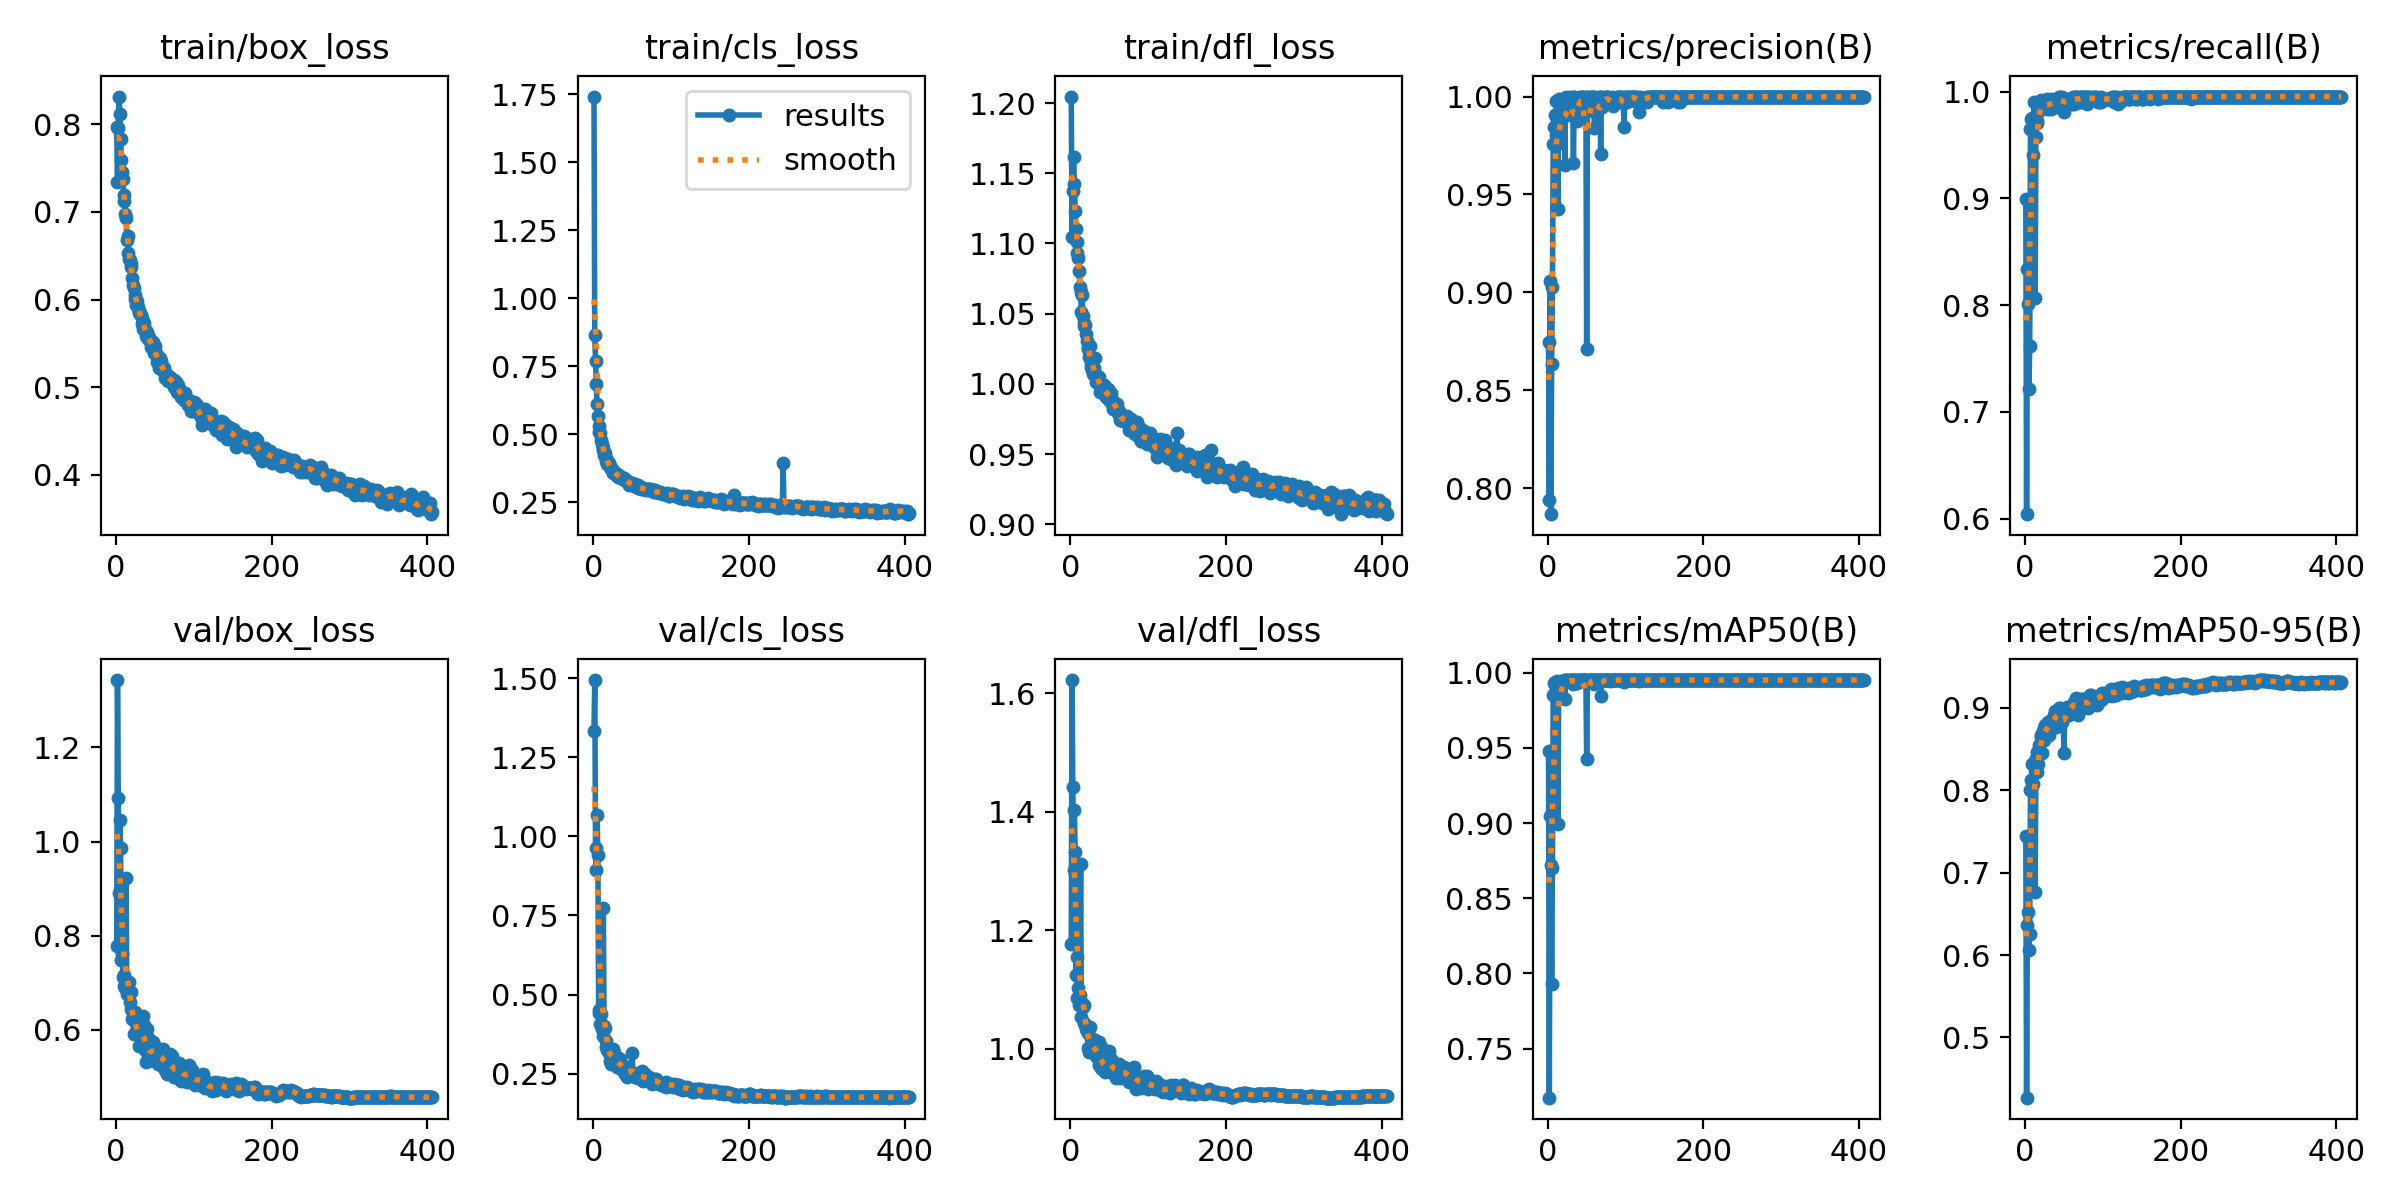
\includegraphics[width=0.95\textwidth]{obrazky-figures/results.png} \caption{Grafy znázorňující vývoj výkonu modelu \texttt{YOLO11n} v~jednotlivých epochách během trénování.} \label{results} \end{figure}

Trénování probíhalo na grafické kartě NVIDIA GeForce GTX 1660 Super, což významně urychlilo výpočty. Použitý počítač byl vybaven procesorem Intel Core i5-9400F a~operační pamětí 16~GB RAM. Po natrénování byl model uložen a~připraven k~použití v~dalších částech systému, kde zajišťuje automatické nalezení oblasti čenichu v~každém vstupním obrázku. Tato detekce je následně využita jako vstup pro výřez relevantní oblasti, která je dále zpracována v~rámci identifikace jedince.


\section{Generování příznakových vektorů pro rozpoznávání}
\label{genEmbedding}
Po úspěšném natrénování detekčního modelu následuje fáze generování embeddingů. V~této fázi model vytváří vektorové reprezentace vyříznutých oblastí čenichu, které slouží k~identifikaci jednotlivých krav v~databázi. Cílem je naučit model generovat takové vektory, aby ty odpovídající snímkům téže krávy byly navzájem umístěny co nejblíže, zatímco vektory snímků různých krav byly od sebe dostatečně vzdálené. To umožňuje spolehlivou identifikaci jednotlivců v~systému a~efektivní porovnávání nových snímků s~již uloženými záznamy.

\subsection*{Příprava dat}
 Nejprve skript využívající detektor čenichů automaticky vyřízl oblast čenichu z~každého obrázku, výřezy byly následně standardizovány na rozměr \(256 \times 256\) pixelů. To zajišťuje, že model bude trénován pouze na relevantních částech obrázků, čímž se eliminuje vliv nežádoucího pozadí a~dalších rušivých faktorů. Pro ověření schopnosti modelu rozpoznat i~nově přidané jedince bylo několik celých tříd vyčleněno. Zbývající data byla náhodně rozdělena na trénovací (70~\%), validační (15~\%) a~testovací (15~\%) sadu. Tento přístup umožňuje objektivně hodnotit výkonnost modelu na neznámých vzorcích a~simulovat reálné scénáře, kdy jsou do systému přidáváni noví jedinci.

\subsection*{Architektura modelu}
Pro generování embeddingů byly využity předtrénované klasifikační neuronové sítě, které byly upraveny odstraněním původní klasifikační vrstvy a~nahrazením novou plně propojenou vrstvou s~výstupem o~velikosti 256~prvků. Ověřeny byly architektury ResNet-50, MobileNet\_V3\_Large a~EfficientNet\_B1, které byly vybrány pro jejich dobrou schopnost extrahovat důležité rysy z~obrazových dat. Výstupní vektory jsou následně normalizovány, to umožňuje efektivní měření vzdáleností mezi embeddingy pomocí eukleidovské vzdálenosti.


\subsection*{Triplet Loss}

Model byl trénován pomocí ztrátové funkce \texttt{TripletMarginLoss}\footnote{\url{https://pytorch.org/docs/stable/generated/torch.nn.TripletMarginLoss.html}}, jejíž princip je popsán v~sekci~\ref{tripletLoss}. 
Matematicky je ztráta definována rovnicí~\ref{loss}.

\begin{equation}
	L(a,p,n) = \max \left\{ d(a_i, p_i) - d(a_i, n_i) + \text{margin}, 0 \right\}
	\label{loss}
\end{equation}

V~rovnici~\ref{loss} proměnné $a$, $p$ a~$n$ označují embeddingy referenčního (\textit{anchor}), pozitivního (\textit{positive}) a~negativního (\textit{negative}) příkladu. Funkce $d$ představuje vzdálenost mezi těmito embeddingy. V~tomto případě je použita eukleidovská vzdálenost, jak je definováno v~rovnici~\ref{distance}. Hodnota \textit{margin} určuje minimální požadovaný rozdíl mezi vzdálenostmi pozitivní a~negativní dvojice. Pokud je rozdíl menší než margin, ztráta je kladná a~model se ji snaží dále minimalizovat. Pro trénování byla hodnota \textit{margin} nastavena na 0,5, což poskytuje dostatečnou hranici pro správné rozeznání rozdílů mezi pozitivními a~negativními dvojicemi.

\begin{equation}
	d(x_i, y_i) = \|x_i - y_i\|_2
	\label{distance}
\end{equation}

\subsection*{Triplet Dataset}
Pro trénování modelu byl vytvořen vlastní \texttt{TripletDataset}, který při každém načítání vzorku náhodně vybírá trojice obrázků (\textit{anchor, positive, negative}) z~aktuální dávky. Tento přístup zajišťuje variabilitu tréninkových dat a~zvyšuje schopnost modelu generalizovat na nové případy, čímž zlepšuje robustnost trénování. Trojice jsou vybírány tak, že pozitivní (\textit{positive}) a~referenční obrázek (\textit{anchor}) pocházejí od stejného jedince (z~téže složky), zatímco negativní obrázek (\textit{negative}) pochází od jiného jedince (z~jiné složky). Vytvořené embeddingy jsou následně vyhodnoceny pomocí ztrátové funkce \texttt{TripletMarginLoss}.

Při validaci je přístup odlišný. Pro zajištění konzistentního hodnocení výkonu modelu jsou trojice pro každou položku validační sady pevně definovány. To umožňuje objektivní porovnání výkonu modelu v~jednotlivých epochách bez vlivu náhodného výběru trojic a~poskytuje opakovatelné výsledky během procesu validace.

\subsection*{Optimalizace}

Pro optimalizaci modelu byl použit algoritmus \texttt{Adam}~\cite{adam} s~počáteční hodnotou \textit{learning rate} 0,001, který je určený pro optimalizaci stochastických cílových funkcí. Adam adaptivně upravuje learning rate jednotlivých parametrů na základě odhadů prvního a~druhého momentu gradientu. Je invariantní vůči diagonálnímu škálování (\textit{rescaling}) gradientů a~dobře se hodí pro problémy s~velkým množstvím dat, řídkými a~hlučnými gradienty, které jsou typické pro trénink embeddingových modelů. Díky intuitivním hyperparametrům a~malé potřebě ladění je Adam ideální volbou pro tento typ úloh.

 Použití plánovače \texttt{ReduceLROnPlateau}\footnote{\url{https://docs.pytorch.org/docs/stable/generated/torch.optim.lr_scheduler.ReduceLROnPlateau.html}} umožnilo dynamicky upravovat \textit{learning rate} během trénování. Pokud validační ztráta nevykazovala po pěti epochách zlepšení, došlo ke snížení \textit{learning rate} na polovinu, to pomáhá modelu v~pozdějších fázích tréninku jemněji konvergovat k~optimálnímu řešení.

\subsection*{Trénování}
Maximální počet epoch byl nastaven na 100. Pro omezení rizika přetrénování byl použit mechanismus včasného zastavení (\textit{early stopping}) s~parametrem \textit{patience} 10, což znamená ukončení trénování v~případě, že se validační ztráta nezlepšila během deseti po sobě jdoucích epoch. Tento přístup pomáhá zabránit tomu, aby se model příliš specializoval na tréninková data na úkor schopnosti generalizace.

Velikost dávky (\textit{batch size}) byla nastavena na 16. Hodnota představuje kompromis mezi stabilitou aktualizací vah modelu a~výpočetní náročností trénování. Příliš malé dávky mohou způsobit vysokou variabilitu gradientů, zatímco příliš velké dávky zvyšují paměťové nároky.

Modely byly trénovány s~využitím předtrénovaných vah extraktorů příznaků na ImageNetu (konkrétně varianty \texttt{IMAGENET1K\_V2} ze standardní distribuce knihovny PyTorch). Trénování probíhalo na grafické kartě NVIDIA GeForce GTX 1660 Super. Použitý počítač byl vybaven procesorem Intel Core i5-9400F a~operační pamětí 16~GB RAM.
Byly natrénovány tři modely na základě odlišných architektur: 
\begin{itemize} 
	\item \textbf{ResNet-50}: Trénování trvalo 81~epoch, nejlepší model byl získán v~71.~epoše s~minimální dosaženou validační ztrátou 0,005. 
	\item \textbf{MobileNet\_V3\_Large}: Trénování probíhalo 61~epoch, nejlepší model byl získán v~51.~epoše s~minimální validační ztrátou 0,0026. 
	\item \textbf{EfficientNet\_B1}: Trénování trvalo 45~epoch, nejlepší model byl získán v~35.~epoše s~minimální validační ztrátou 0,005. \end{itemize}

Během trénování byla průběžně sledována tréninková i~validační ztráta, aby bylo možné vyhodnotit stabilitu učení, průběh konvergence a~včas detekovat případné problémy. Úspěšnost jednotlivých modelů bude analyzována v~kapitole~\ref{kap5}, která se zaměří na experimentální ověření kvality identifikace.


\section{Uživatelské rozhraní}
\label{gui}
Pro praktické využití trénovaného systému byla vytvořena desktopová aplikace s~grafickým uživatelským rozhraním (GUI). Aplikace byla navržena tak, aby byla intuitivní, snadno ovladatelná a~dostatečně flexibilní pro rozšiřování o~nové funkce. Rozhraní nabízí dvě základní funkce: identifikaci, tedy určení identity jedince na základě vstupního snímku čenichu, a~verifikaci, která slouží k~ověření, zda dva snímky patří téže krávě. Aplikace využívá dříve popsané komponenty systému (model pro detekci čenichu a~model pro výpočet vektorové reprezentace snímku) a~spojuje je do uceleného nástroje, který umožňuje snadné nasazení systému v~reálných podmínkách.

\subsection*{Identifikační režim}
V identifikačním režimu (viz obrázek~\ref{identifycationApp}) uživatel vloží snímek čenichu libovolné krávy. Po kliknutí na tlačítko \textit{Identify} pod obrázkem dojde k~automatické detekci oblasti čenichu, která je vyznačena rámečkem v~původním obrázku. Následně se z~této oblasti vytvoří embedding a~ten je porovnán se všemi embeddingy v~databázi. Na základě eukleidovské vzdálenosti se určí nejbližší soused a~zobrazí se identita odpovídající krávy. Pokud vzdálenost k~nejbližšímu vektoru překročí předem nastavený rozhodovací práh, je uživateli oznámeno, že daný jedinec se v~databázi pravděpodobně nenachází.

\begin{figure}[hbt]
	\centering
	\includegraphics[width=0.65\textwidth]{obrazky-figures/identification\_app.png}
	\caption{Identifikační režim aplikace pro identifikaci krávy na základě snímku čenichu, kde je znázorněna detekovaná oblast čenichu a~zobrazena identita dané krávy.}
	\label{identifycationApp}
\end{figure}

\subsection*{Verifikační režim}
Verifikační režim (viz obrázek~\ref{verificationApp}) slouží k~porovnání dvou snímků a~určení, zda zobrazují stejného jedince. Uživatel vloží dvě fotografie a~po stisknutí tlačítka \textit{Verify} pod obrázky aplikace v~každém z~nich automaticky detekuje oblast čenichu. Tyto oblasti jsou označeny rámečky a~z~každé je následně vytvořen embedding. Porovnáním obou embeddingů pomocí eukleidovské vzdálenosti se rozhodne, zda se jedná o~stejnou krávu nebo dvě různé krávy. Toto rozhodnutí je řízeno prahovou hodnotou.

\begin{figure}[hbt]
	\centering
	\includegraphics[width=0.65\textwidth]{obrazky-figures/verification\_app.png}
	\caption{Verifikační režim aplikace pro porovnání dvou snímků, kde jsou znázorněny detekované oblasti čenichu na obou snímcích, a~rozhodnutí, že krávy nejsou stejné.}
	\label{verificationApp}
\end{figure}


\subsection*{Nastavení}
Aplikace ve výchozím nastavení používá model a~prahovou hodnotu, které byly v~experimentální části (viz sekce~\ref{bestModel}) vyhodnoceny jako nejlepší. Uživatel má však možnost tyto parametry v~nastavení aplikace libovolně měnit. Lze zvolit jiný model z~nabídky dostupných architektur (ResNet-50, MobileNet\_V3\_Large nebo EfficientNet\_B1) a~upravit hodnotu prahu, který se používá k~rozhodování v~obou režimech. 

Při změně modelu se do databáze automaticky nahrají embeddingy vytvořené daným modelem, které jsou předem připravené. Tím je zajištěna konzistence mezi databází a~aktuálně používaným modelem bez nutnosti zdlouhavého přepočtu embeddingů. Tato flexibilita umožňuje snadné přizpůsobení chování systému různým podmínkám, například při testování jiných modelových konfigurací nebo v~případě specifických požadavků na citlivost identifikace a~verifikace.

Kromě toho lze v~nastavení povolit zobrazení vypočtené vzdálenosti mezi embeddingy. V~identifikačním režimu je tím myšlena vzdálenost mezi vloženým obrázkem a~nejbližším embeddingem v~databázi, zatímco ve verifikačním režimu se zobrazuje vzdálenost mezi embeddingy vypočtenými ze dvou zadaných snímků.

\chapter{Experimenty a~analýza výsledků}
\label{kap5}
Tato kapitola se zabývá vyhodnocením přesnosti a~praktické použitelnosti řešení pro identifikaci skotu na základě snímků čenichu. Systém se skládá ze dvou hlavních částí (detektoru čenichu a~identifikačního modelu). V~první fázi je ověřována přesnost detekčního modelu, který slouží k~automatickému ořezání relevantní části snímku. Následně je hodnocena schopnost jednotlivých identifikačních modelů rozlišit mezi různými jedinci a~spolehlivě rozhodnout, zda dotazovaný snímek odpovídá některému ze známých zvířat, nebo zda se jedná o~zcela nový, dosud neidentifikovaný případ.

V rámci experimentální části byly porovnávány tři architektury neuronových sítí upravené pro extrakci embeddingů (ResNet-50, MobileNet\_V3\_Large a~EfficientNet\_B1). \linebreak Všechny modely byly trénovány na shodné trénovací množině obsahující výřezané snímky čenichů krav a~jejich výstupem jsou vektorové reprezentace (embeddingy), které se následně normalizují a~porovnávají pomocí eukleidovské vzdálenosti. Ta pro dva embeddingy \texttt{a} a~\texttt{b} určuje délku jejich rozdílového vektoru podle rovnice~\ref{euclidean}~\cite{Precision}.

\begin{equation}
	d(a, b) = \sqrt{\sum_{i=1}^{n} (a_i - b_i)^2}
	\label{euclidean}
\end{equation}

Tato metrika umožňuje kvantifikovat podobnost mezi dvěma snímky. Čím menší je vzdálenost mezi embeddingy, tím vyšší je pravděpodobnost, že snímky reprezentují stejnou krávu.

Pro účely vyhodnocení byla vytvořena databáze embeddingů, která obsahuje vektory všech snímků krav z~trénovací sady. Dotazovací množina (\textit{test set}) je složena z~odlišných snímků a~zahrnuje jak jedince, kteří byli při trénování zastoupeni (známé krávy), tak i~jedince, kteří se v~trénovacích datech nevyskytují (neznámé krávy). Tento testovací scénář odpovídá praktickému nasazení systému, ve kterém může být každý dotaz novým zvířetem nebo opakovaným výskytem již registrovaného jedince.

Účelem testování je vyhodnotit jak přesnost detekce čenichu, tak schopnost systému spolehlivě rozhodovat na základě porovnání vektorových výstupů modelu. Nejprve jsou představeny metriky, které jsou využívány v~jednotlivých experimentech. První část testování ověřuje přesnost detektoru. Následuje analýza vzdáleností mezi vektorovými reprezentacemi snímků od stejných a~různých jedinců. Další experimenty se zaměřují na volbu vhodného rozhodovacího prahu -- nejprve na základě dosažené přesnosti, následně podle vyvážené přesnosti. Závěrečný experiment hodnotí schopnost modelu generalizovat na dosud neznámé jedince a~opět analyzuje vzdálenosti i~úspěšnost rozhodování při různých hodnotách prahu.

\section{Metriky}
\label{metrics}
Při vyhodnocování přesnosti systému byly využity různé metriky, které odpovídají specifickým cílům jednotlivých fází zpracování a~experimentů. Vzhledem k~tomu, že navržený systém kombinuje dva odlišné úkoly (detekci čenichu a~identifikaci jednotlivých jedinců), je nutné volit metody hodnocení tak, aby adekvátně reflektovaly požadované vlastnosti každé části. Pro detekční část jsou použity standardní metriky objektové detekce, které posuzují schopnost modelu lokalizovat čenich ve snímku s~dostatečnou přesností a~konzistencí. V~identifikační části je pak hodnocena schopnost systému správně přiřadit identitu na základě vektorových reprezentací, přičemž se bere v~potaz i~případné odmítnutí neznámých jedinců.

\subsection*{Metriky pro hodnocení detekce}
Pro vyhodnocení kvality modelu pro detekci čenichu jsou použity standardní metriky využívané v~oblasti objektové detekce~\cite{yolo_docs}:
\begin{itemize}
	\item \textbf{Precision}: Podíl správně detekovaných objektů mezi všemi detekcemi.
	\item \textbf{Recall}: Podíl správně detekovaných objektů mezi všemi skutečně se vyskytujícími.
	\item \textbf{F1 skóre}: Harmonický průměr \textit{precision} a~\textit{recall}.
	\item \textbf{mAP50}: Průměrná přesnost při prahové hodnotě překrytí (\textit{IoU}) 0,5.
	\item \textbf{mAP50-95}: Průměrná přesnost napříč hodnotami \textit{IoU} v~rozsahu 0,5--0,95.
\end{itemize}

\subsection*{Metriky pro hodnocení identifikace}
Pro vyhodnocení identifikační části systému jsou využity klasifikační metriky, jejichž výběr a~matematické definice vycházejí ze shrnutí uvedeného ve zdroji~\cite{lossMetrics}. Formulace jednotlivých pojmů byla přizpůsobena specifikům úlohy rozpoznávání jednotlivých krav. Tyto metriky pracují se čtyřmi základními typy rozhodnutí:

\begin{itemize}
	\item \textbf{True Positive (TP)}: Známý jedinec byl správně identifikován.
	\item \textbf{False Positive (FP)}: Neznámý jedinec byl chybně přiřazen k~některé známé krávě.
	\item \textbf{True Negative (TN)}: Neznámý jedinec byl správně odmítnut.
	\item \textbf{False Negative (FN)}: Známý jedinec byl nesprávně odmítnut, protože jeho embedding byl považován za příliš vzdálený od vzorů v~databázi.
\end{itemize}
Z těchto hodnot byly spočítány následující metriky:
\begin{itemize}
	\item \textbf{Accuracy}: Podíl všech správně klasifikovaných případů (rozpoznaných známých i~odmítnutých neznámých) z~celkového počtu všech případů (viz rovnice~\ref{accuracy}).
	\begin{equation}
		\text{Accuracy} = \frac{TP + TN}{TP + TN + FP + FN}
		\label{accuracy}
	\end{equation}
	
	\item \textbf{True Positive Rate (TPR, Recall)}: Podíl známých jedinců, kteří byli správně rozpoznáni, z~celkového počtu všech známých jedinců (viz rovnice~\ref{recall}).
	\begin{equation}
		\text{TPR} = \frac{TP}{TP + FN}
		\label{recall}
	\end{equation}
	
	\item \textbf{Precision}: Podíl správně rozpoznaných známých jedinců z~celkového počtu všech případů, kdy model označil jedince jako známého (viz rovnice~\ref{precision}).
	\begin{equation}
		\text{Precision} = \frac{TP}{TP + FP}
		\label{precision}
	\end{equation}
	
	\item \textbf{True Negative Rate (TNR, Specificity)}: Podíl neznámých jedinců, kteří byli správně odmítnuti, z~celkového počtu všech neznámých jedinců (viz rovnice~\ref{specificity}).
	\begin{equation}
		\text{TNR} = \frac{TN}{TN + FP}
		\label{specificity}
	\end{equation}

	\item \textbf{Balanced Accuracy}: Tato metrika slouží ke zmírnění vlivu nevyváženosti tříd tím, že každé třídě přiřazuje stejnou váhu. Zatímco ve vícetřídových úlohách se počítá jako průměr hodnot \textit{recall} napříč jednotlivými třídami, v~případě binární klasifikace použité v~této práci (známý vs. neznámý jedinec) odpovídá průměru TPR a~TNR (viz rovnice~\ref{balancedAcc}).
	\begin{equation}
		\text{Balanced Accuracy} = \frac{1}{2} (\text{TPR} + \text{TNR})
		\label{balancedAcc}
	\end{equation}
\end{itemize}

\section{Testování přesnosti detekce}
\label{testDetector}
Pro ověření kvality trénovaného modelu detekce čenichu byla provedena evaluace na testovací množině dat, která nebyla během trénování využita.
K hodnocení byly využity standardní metriky uvedené v~sekci~\ref{metrics}, konkrétně \textit{precision}, \textit{recall}, \textit{mAP50} a~\textit{mAP50-95}. Tyto ukazatele dohromady poskytují komplexní pohled na výkon detektoru. Výsledky dosažené modelem svědčí o~jeho vysoké přesnosti i~schopnosti generalizace:
\begin{itemize}
	\item \textbf{Precision} = 1: Všechny detekce modelu byly správné.
	\item \textbf{Recall} = 1: Model detekoval všechny čenichy.
	\item \textbf{mAP50} = 0,995: Model vykazuje velmi vysokou přesnost lokalizace při standardní prahové hodnotě \textit{IoU} 0,5.
	\item \textbf{mAP50-95} = 0,937: Model je robustní napříč různými úrovněmi překrytí (\textit{IoU} práh od 0,5 do 0,95).
\end{itemize}

Důležitým doplňkem těchto ukazatelů je také hodnocení pomocí F1 skóre, které představuje harmonický průměr \textit{precision} a~\textit{recall}, a~tudíž poskytuje jednotný pohled na rovnováhu mezi těmito dvěma aspekty výkonu. F1 křivka, znázorněná na obrázku~\ref{f1_curve}, demonstruje chování tohoto skóre při různých hodnotách prahu detekce. Stabilně vysoké hodnoty F1 skóre potvrzují spolehlivost modelu a~jeho schopnost dobře balancovat mezi úplností detekce a~její přesností.

\begin{figure}[hbt]\centering
	\centering
	\includegraphics[width=0.6\textwidth]{obrazky-figures/F1\_curve.png}
	\caption{F1 křivka výsledného modelu znázorňuje vztah mezi prahovou hodnotou detekce a~výkonem modelu.}
	\label{f1_curve}
\end{figure}

Kromě číselného vyhodnocení byly výsledky testování podpořeny také vizuální kontrolou. Za tímto účelem byly vygenerovány snímky s~predikcemi modelu označené jako \texttt{val\_batch\_pred}, které zobrazují pozice čenichů detekované modelem formou ohraničujících rámečků. Tyto vizualizace umožňují rychle zhodnotit, zda model skutečně rozpoznává čenichy správně i~z~lidského pohledu. Ukázka části takového výstupu je uvedena na obrázku~\ref{val_batch_pred}.

Celkové výsledky ukazují, že detektor čenichů dosahuje vysoké přesnosti i~spolehlivosti a~je připraven být nasazen jako vstupní komponenta do systému identifikace jednotlivých krav.

\begin{figure}[hbt]
	\centering
	\includegraphics[width=0.9\textwidth]{obrazky-figures/val\_batch\_pred.png}
	\caption{Část snímku získaného při testování \texttt{YOLO11n}, který ukazuje predikce modelu.}
	\label{val_batch_pred}
\end{figure}


\section{Analýza vzdáleností mezi embeddingy}
\label{distanceMetrics}
Cílem tohoto experimentu bylo analyzovat rozložení vzdáleností mezi embeddingy dotazovaných snímků a~embeddingy uloženými v~databázi. Tato analýza poskytuje základní přehled o~tom, jak dobře model rozlišuje snímky krav, které již v~databázi jsou (pozitivní případy), od těch, které se v~databázi nevyskytují (negativní případy).

Pro každý dotazovaný snímek byl v~databázi vyhledán embedding s~nejmenší eukleidovskou vzdáleností. Pokud tento embedding odpovídal stejné krávě jako dotazovaný snímek, jednalo se o~pozitivní případ; v~opačném případě šlo o~negativní případ. Cílem tohoto postupu nebylo rozhodnout, zda se konkrétní snímek v~databázi již nachází, ale pouze zaznamenat, jak se liší vzdálenosti mezi embeddingy v~závislosti na správnosti přiřazení. Tato analýza umožňuje získat základní přehled o~kvalitě embeddingového prostoru a~poskytuje první indikaci o~tom, jaká hodnota prahu by mohla být vhodná pro následné rozhodování, zda je dotazovaný snímek v~databázi zastoupen. Pro každý testovaný model byly následně vypočteny následující charakteristické hodnoty:

\begin{itemize} 
	\item Průměrná vzdálenost při správné identifikaci -- tedy mezi embeddingy patřícími stejné krávě. 
	\item Průměrná vzdálenost při chybné identifikaci -- tedy mezi embeddingy různých krav. 
	\item Největší vzdálenost mezi embeddingy, při které došlo ke správné identifikaci -- reprezentuje nejméně přesný pozitivní případ. 
	\item Nejmenší vzdálenost mezi embeddingy, při které došlo k~chybné identifikaci -- představuje nejvíce matoucí negativní případ. 
\end{itemize}

Výsledné hodnoty pro jednotlivé modely shrnuje tabulka~\ref{distances}.

\renewcommand{\arraystretch}{1.3}
\begin{table}[H]
	\centering
	\begin{tabular}{|c|c|c|c|c|}
		\hline
		\multirow{2}{*}{\textbf{Model}} & 
		\multicolumn{2}{c|}{\parbox[c][3em][c]{4.5cm}{\centering \textbf{Vzdálenosti}\\\textbf{pozitivních případů}}} & 
		\multicolumn{2}{c|}{\parbox[c][3em][c]{4.5cm}{\centering \textbf{Vzdálenosti}\\\textbf{negativních případů}}} \\
		\cline{2-5}
		& \textbf{\centering Průměr} & \textbf{\centering Maximální} & \textbf{\centering Průměr} & \textbf{\centering Minimální} \\
		\hline
		EfficientNet\_B1 & 0,1394 & 0,5843 & 0,4324 & 0,0662 \\
		MobileNet\_V3\_Large & 0,1695 & 0,6766 & 0,5106 & 0,0666 \\
		ResNet-50 & 0,1716 & 0,7075 & 0,5002 & 0,0662 \\
		\hline
	\end{tabular}
	\caption{Přehled vzdáleností mezi embeddingy dotazovaných snímků a~nejbližšími uloženými vzory pro případy správného (pozitivního) a~nesprávného (negativního) přiřazení.}
	\label{distances}
\end{table}

Graf na obrázku~\ref{hist-efficientnet} zobrazuje rozložení vzdáleností mezi embeddingy ve dvojicích, kde oba snímky náleží stejné krávě (\textit{genuine pairs}), a~ve dvojicích různých krav (\textit{impostor pairs}) pro EfficientNet\_B1. Je vidět, že většina vzdáleností mezi embeddingy stejné krávy je soustředěna kolem nižších hodnot a~vzdálenosti mezi embeddingy různých krav jsou vyšší, ačkoliv se rozložení částečně překrývají. To podtrhuje význam správné volby prahu.
\begin{figure}[H]
	\centering
	\includegraphics[width=0.8\textwidth]{obrazky-figures/genuine\_impostor\_classification\_efficientnetb1.pdf}
	\caption{Rozložení vzdáleností mezi embeddingy pro model EfficientNet\_B1.}
	\label{hist-efficientnet}
\end{figure}

Obdobné histogramy byly vytvořeny i~pro architektury MobileNet\_V3\_Large a~ResNet-50 (viz obrázek~\ref{hist-mobilenet} a~\ref{hist-resnet}). U~všech modelů lze pozorovat určitý překryv mezi \textit{genuine} a~\textit{impostor} dvojicemi. To znamená, že žádný model není zcela jednoznačný ve své rozhodovací hranici.

\begin{figure}[H]
	\centering
	\includegraphics[width=0.8\textwidth]{obrazky-figures/genuine\_impostor\_classification\_mobilenet.pdf}
	\caption{Rozložení vzdáleností mezi embeddingy pro model MobileNet\_V3\_Large.}
	\label{hist-mobilenet}
\end{figure}

\begin{figure}[H]
	\centering
	\includegraphics[width=0.8\textwidth]{obrazky-figures/genuine\_impostor\_classification\_resnet.pdf}
	\caption{Rozložení vzdáleností mezi embeddingy pro model ResNet-50.}
	\label{hist-resnet}
\end{figure}

Z výsledků je patrné, že model EfficientNet\_B1 vykazuje nejnižší hodnoty jak průměrné vzdálenosti v~pozitivních případech (0,1394), tak i~maximální vzdálenosti při správné identifikaci (0,5843). To naznačuje, že embeddingy vytvářené tímto modelem jsou v~rámci jednoho jedince konzistentnější a~lépe soustředěné, což by mohlo umožnit použití nižšího rozhodovacího prahu bez výrazného rizika chybných negativních rozhodnutí.

Naopak v~případě modelů MobileNet\_V3\_Large a~ResNet-50 lze pozorovat vyšší hodnoty jak v~průměrné, tak v~maximální vzdálenosti mezi správně identifikovanými případy (MobileNet\_V3\_Large 0,6766, ResNet-50 0,7075). Tyto modely jsou tedy méně konzistentní, co se týče rozmístění embeddingů pro stejného jedince. To může znamenat, že pro správnou identifikaci bude třeba zvolit vyšší prahovou hodnotu. Zároveň mají ale vyšší průměrné vzdálenosti v~negativních případech než EfficientNet\_B1, což by mohlo usnadnit odlišení nových krav, které v~databázi nejsou.

Zajímavé je, že minimální vzdálenosti v~negativních případech jsou téměř totožné napříč všemi modely (kolem 0{,066}). To ukazuje, že některé embeddingy neznámých krav se velmi těsně přibližují známým vzorům v~databázi. Tato skutečnost omezuje maximální bezpečný práh pro detekci nových jedinců. Pokud by byl práh nastaven příliš vysoko, hrozí falešná identifikace i~v~negativních případech.

Celkově tedy tato analýza ukazuje, že volba vhodného rozhodovacího prahu by měla zohledňovat nejen průměrné vzdálenosti, ale i~extrémní hodnoty. Například pro EfficientNet\_B1 by bylo možné použít nižší práh, zatímco pro modely ResNet-50 nebo MobileNet\_V3\_Large by měl být práh nastaven výše, pokud chceme dosáhnout plného pokrytí pozitivních případů. Je však důležité si uvědomit, že příliš vysoká hodnota prahu sice může zajistit, že všechny snímky známých krav budou správně identifikovány, ale zároveň zvyšuje riziko, že neznámý jedinec bude nesprávně přiřazen k~některé z~krav v~databázi. V~dalším experimentu bude právě vliv volby hodnoty prahu na celkovou přesnost vyhodnocen podrobněji.


\section{Testování prahových hodnot}
\label{threshold}
V této části hodnotíme úspěšnost identifikace jednotlivých jedinců v~závislosti na nastavené prahové hodnotě maximální přípustné vzdálenosti mezi embeddingy. Nejprve se zaměřujeme na celkovou přesnost, to sice poskytne přehled o~chování modelu na konkrétním testovacím datasetu, ale vzhledem k~nevyváženosti tříd (výrazně více pozitivních než negativních vzorků) tato metrika nemusí plně vystihovat skutečnou kvalitu modelu. Proto v~druhé části využíváme vyváženou úspěšnost (\textit{balanced accuracy}), která poskytuje objektivnější pohled na chování modelu napříč třídami.

\subsection*{Vyhodnocení pomocí přesnosti}
\label{bestModel}
Identifikace jednotlivých jedinců byla testována při různých prahových hodnotách. Pro každý model byla při daném prahu vyhodnocena přesnost, která udává, jaká část testovacích případů byla správně klasifikována (tedy jako true positive nebo true negative). Ačkoliv se jedná o~jednoduchou a~intuitivní metriku, v~tomto případě není zcela vhodná pro jednoznačné hodnocení kvality identifikačního systému. Důvodem je výrazná nevyváženost tříd v~testovacím datasetu -- pozitivních případů (tedy známých jedinců) je výrazně více než negativních (neznámých jedinců). Tento nepoměr může vést k~nadhodnocení výsledků, protože i~model, který by neodmítl žádného neznámého jedince, by mohl mít vysokou přesnost, pokud by správně identifikoval většinu známých jedinců.

Přestože je tato metrika omezená kvůli nevyváženosti tříd, může posloužit jako hrubý odhad úspěšnosti modelů a~jako výchozí bod pro výběr výchozího nastavení v~uživatelském rozhraní. Tento výběr je důležitý, protože aplikace bude primárně testována na tomto specifickém datasetu, kde se očekává, že model bude úspěšný v~identifikaci známých jedinců. V~reálném nasazení, kde může být třída známých a~neznámých jedinců vyváženější, by však bylo žádoucí použít jiné metriky, jako je například \textit{recall} nebo \textit{specificity}, které lépe zohlední rovnováhu mezi třídami a~kvalitu detekce obou kategorií. Tyto metriky budou podrobněji analyzovány v~následujícím experimentu.

V tabulce~\ref{tab:results} jsou uvedeny výsledky testování tří modelů (EfficientNet\_B1, MobileNet\_V3\_Large a~ResNet-50) při různých prahových hodnotách. Pro každý model je v~tabulce zvýrazněna nejlepší dosažená přesnost. Z~těchto výsledků je patrné, že model MobileNet\_V3\_Large dosáhl nejvyšší přesnosti s~prahovou hodnotou 0,5, kdy dosáhl hodnoty 0,9581. Tento model tedy vykazuje nejlepší výkon v~rámci testovaného datasetu při použití tohoto prahu.
\begin{table}[h!]
	\centering
	\begin{tabular}{|c|c|c|c|}
		\hline
		\textbf{Threshold} & \textbf{EfficientNet\_B1} & \textbf{MobileNet\_V3\_Large} & \textbf{ResNet-50} \\ \hline
		0,4 & 0,9354 & 0,9332 & 0,9112 \\ \hline
		0,5 & \textbf{0,9446} & \textbf{0,9581} & 0,9276 \\ \hline
		0,6 & 0,9411 & 0,9560 & \textbf{0,9332} \\ \hline
		0,7 & 0,9354 & 0,9489 & 0,9261 \\ \hline
		0,8 & 0,9354 & 0,9460 & 0,9247 \\ \hline
	\end{tabular}
	\caption{Výsledky modelů při různých prahových hodnotách. Zvýrazněna vždy nejvyšší dosažená přesnost daného modelu.}
	\label{tab:results}
\end{table}

\subsection*{Vyhodnocení pomocí vyvážené přesnosti (Balanced Accuracy)}
Vzhledem k~výrazné nevyváženosti tříd v~testovacím datasetu, kdy převažují pozitivní případy (snímky známých jedinců) nad případy negativními (snímky neznámých jedinců), nelze spoléhat pouze na celkovou přesnost jako hlavní ukazatel výkonnosti identifikačního systému. Přesnost totiž může být vysoká i~v~případě, že model špatně pracuje s~menšinovou třídou, což je v~reálném nasazení nežádoucí.

Z tohoto důvodu se hodnocení zaměřuje na podrobnější metriky, které lépe vystihují schopnost modelu rozlišovat mezi oběma třídami. Konkrétně jsou sledovány hodnoty \textit{True Positive Rate (TPR)} a~\textit{True Negative Rate (TNR)}, které udávají úspěšnost rozpoznání pozitivních a~negativních případů. Tyto dvě metriky jsou následně zprůměrovány do složené metriky \textit{balanced accuracy}, která poskytuje vyvážený pohled na klasifikační výkon modelu bez ohledu na poměr tříd v~testovacích datech.

Metrika \textit{balanced accuracy} je obzvláště vhodná pro případy, kdy je žádoucí, aby systém dosahoval srovnatelné úspěšnosti při správné identifikaci známých jedinců i~při správném odmítnutí těch neznámých. Vyšší hodnota této metriky svědčí o~rovnoměrné výkonnosti modelu napříč oběma kategoriemi případů. Je důležité si zároveň uvědomit, že práh rozhodování, který maximalizuje \textit{balanced accuracy}, nemusí být totožný s~tím, který poskytuje nejvyšší běžnou přesnost (\textit{accuracy}). Při výběru vhodného prahu je však právě \textit{balanced accuracy} vhodnějším kritériem, protože eliminuje vliv nevyváženého zastoupení tříd.

Pro každý testovaný model byla sestavena samostatná tabulka, která uvádí hodnoty metrik TPR, TNR a~\textit{balanced accuracy} pro různé hodnoty rozhodovacího prahu. Pro přehlednost je v~každé tabulce zvýrazněna nejvyšší dosažená hodnota \textit{balanced accuracy} a~tabulka vždy pokrývá i~její bezprostřední okolí. Tímto způsobem je možné sledovat chování jednotlivých modelů v~závislosti na rozhodovacím prahu a~podpořit informované rozhodnutí o~jeho vhodném nastavení pro budoucí nasazení systému.




\subsubsection*{EfficientNet\_B1}
Tabulka~\ref{efficientnetMetrics} shrnuje hodnoty TPR, TNR a~\textit{balanced accuracy} dosažené modelem EfficientNet\_B1 při různých prahových hodnotách. Nejvyšší \textit{balanced accuracy} zde bylo dosaženo při prahu 0,24, a~to s~hodnotou 0,8367. Zajímavé je, že model si udržuje poměrně stabilní TNR i~TPR v~okolí této hodnoty. To může být výhodou při praktickém nasazení, kde se mírné odchylky v~prahu nemusí významně projevit na výkonnosti. Celkově však \textit{balanced accuracy} zůstává o~něco nižší než u~ostatních dvou modelů.


\begin{table}[h!]
	\centering
	\begin{tabular}{|c|c|c|c|}
		\hline
		\textbf{Threshold} & \textbf{TPR} & \textbf{TNR} & \textbf{Balanced Accuracy} \\ \hline
		0,21 & 0,8078 & 0,8400 & 0,8239 \\ \hline
		0,23 & 0,8409 & 0,8200 & 0,8305 \\ \hline
		0,24 & 0,8535 & 0,8200 & \textbf{0,8367} \\ \hline
		0,25 & 0,8651 & 0,8039 & 0,8345 \\ \hline
		0,27 & 0,8819 & 0,7736 & 0,8278 \\ \hline
	\end{tabular}
	\caption{Hodnoty TPR, TNR a~balanced accuracy pro model EfficientNet\_B1 při různých prahových hodnotách}
	\label{efficientnetMetrics}
\end{table}

\subsubsection*{MobileNet\_V3\_Large}
Výsledky modelu MobileNet\_V3\_Large jsou uvedeny v~tabulce~\ref{mobilenetMetrics}. Tento model dosáhl nejvyšší \textit{balanced accuracy} ze všech testovaných architektur, a~to 0,8814 při prahu 0,33. Hodnoty TPR i~TNR jsou zde velmi vyvážené, to svědčí o~schopnosti modelu správně klasifikovat jak známé, tak neznámé jedince.


\begin{table}[h!]
	\centering
	\begin{tabular}{|c|c|c|c|}
		\hline
		\textbf{Threshold} & \textbf{TPR} & \textbf{TNR} & \textbf{Balanced Accuracy} \\ \hline
		0,30 & 0,8778 & 0,8600 & 0,8689 \\ \hline
		0,32 & 0,8940 & 0,8600 & 0,8770 \\ \hline
		0,33 & 0,9028 & 0,8600 & \textbf{0,8814} \\ \hline
		0,34 & 0,9123 & 0,8431 & 0,8777 \\ \hline
		0,36 & 0,9218 & 0,8269 & 0,8744 \\ \hline
	\end{tabular}
	\caption{Hodnoty TPR, TNR a~balanced accuracy pro model MobileNet\_V3\_Large při různých prahových hodnotách}
	\label{mobilenetMetrics}
\end{table}

\subsubsection*{ResNet-50}
Tabulka~\ref{resnetMetrics} prezentuje výsledky modelu ResNet-50. Nejvyšší \textit{balanced accuracy} zde dosahuje hodnoty 0,8218 při prahové hodnotě 0,32. Oproti MobileNet\_V3\_Large i~EfficientNet\_B1 je zde patrný výraznější rozdíl mezi TPR a~TNR. Model má tendenci více preferovat rozpoznávání známých jedinců, zatímco schopnost správně odmítat neznámé je nižší. Přesto však výsledky nejsou nekonzistentní a~vhodnou volbou prahu lze ResNet-50 také nastavit tak, aby poskytoval přijatelné výsledky. 

\begin{table}[h!]
	\centering
	\begin{tabular}{|c|c|c|c|}
		\hline
		\textbf{Threshold} & \textbf{TPR} & \textbf{TNR} & \textbf{Balanced Accuracy} \\ \hline
		0,29 & 0,8383 & 0,7963 & 0,8173 \\ \hline
		0,31 & 0,8632 & 0,7679 & 0,8155 \\ \hline
		0,32 & 0,8757 & 0,7679 & \textbf{0,8218} \\ \hline
		0,33 & 0,8882 & 0,7544 & 0,8213 \\ \hline
		0,35 & 0,9021 & 0,7167 & 0,8094 \\ \hline
	\end{tabular}
	\caption{Hodnoty TPR, TNR a~balanced accuracy pro model ResNet-50 při různých prahových hodnotách}
	\label{resnetMetrics}
\end{table}

\subsubsection*{Shrnutí výsledků a~srovnání modelů}
V předchozích tabulkách jsme prezentovali výsledky testování tří modelů (EfficientNet\_B1, MobileNet\_V3\_Large a~ResNet-50) při různých prahových hodnotách. Pro každý model byl následně zvolen takový práh, který maximalizoval hodnotu vyvážené přesnosti (\textit{balanced accuracy}). Tento přístup umožňuje zohlednit i~méně zastoupenou třídu neznámých jedinců a~je tak vhodnější pro vyvážené hodnocení výkonu modelu.

Nejvyšší hodnoty \textit{balanced accuracy} (0,8814) dosáhl model MobileNet\_V3\_Large při prahu 0,33, čímž prokázal nejlepší schopnost současně správně identifikovat známé jedince a~správně odmítat ty neznámé. U~ostatních modelů bylo nejlepší vyvážení dosaženo při nižších prahových hodnotách, u~EfficientNet\_B1 při 0,24 a~u~ResNet-50 při 0,32.

Aby bylo možné lépe posoudit, jak si jednotlivé modely vedou v~rámci konkrétního aplikačního scénáře, byla sestavena souhrnná tabulka~\ref{metricsComparison}. Ta hodnotí výkon každého modelu při jeho optimálně zvoleném prahu tentokrát pomocí běžně používaných metrik \textit{accuracy}, \textit{precision} a~\textit{recall}. Výsledky byly získány na testovacím datasetu, ve kterém převažují pozitivní případy (známí jedinci). Tento nerovnoměrný poměr tříd je dán charakterem dostupných dat, a~přestože nereflektuje zcela typické nasazení systému v~praxi, poskytuje cenné informace o~tom, jak spolehlivě je model schopen identifikovat jedince, které už má uložené v~databázi.

\begin{table}[hbt]
	\centering
	\begin{tabular}{|c|c|c|c|c|}
		\hline
		\textbf{Model} & \textbf{Threshold} & \textbf{Recall} & \textbf{Precision} & \textbf{Accuracy} \\ \hline
		EfficientNet\_B1 & 0,24 & 0,8535 & 0,9923 & 0,8523 \\ \hline
		MobileNet\_V3\_Large & 0,33 & 0,9028 & 0,9943 & 0,9013 \\ \hline
		ResNet-50 & 0,32 & 0,8757 & 0,9891 & 0,8714 \\ \hline
	\end{tabular}
	\caption{Metriky pro každý model při prahu vybraném na základě \textit{balanced accuracy}}
	\label{metricsComparison}
\end{table}

Z výsledků je patrné, že nejvyšších hodnot všech tří sledovaných metrik (\textit{recall}, \textit{precision} a~\textit{accuracy}) dosahuje model MobileNet\_V3\_Large při prahové hodnotě 0,33. Tento model správně identifikuje přibližně 90~\% známých jedinců (recall 0,9028) a~zároveň vykazuje velmi nízkou míru falešné identifikace (\textit{precision} 0,9943), což znamená, že téměř všechny pozitivní predikce odpovídají skutečně známým jedincům. Celková přesnost modelu (\textit{accuracy}) je 0,9013. Navíc tento model dosáhl i~nejvyšší hodnoty \textit{balanced accuracy}, která potvrzuje jeho dobrou schopnost vyváženě klasifikovat známé i~neznámé jedince.

Model ResNet-50 při prahové hodnotě 0,32 vykazuje rovněž vysoké hodnoty \textit{recall} (0,8757) a~\textit{accuracy} (0,8714), avšak jeho \textit{balanced accuracy} byla nižší. To naznačuje, že model má tendenci více upřednostňovat klasifikaci případů jako \uv{známý jedinec} a~to může vést k~vyššímu počtu falešných pozitivních identifikací. Jeho celková přesnost tak částečně odráží nevyváženost dat a~nemusí plně vypovídat o~skutečné robustnosti modelu.

Naopak EfficientNet\_B1 dosahuje nejnižší hodnoty \textit{recall} (0,8535) i~\textit{accuracy} (0,8523), ale vykazuje vysokou \textit{precision} (0,9923), která značí konzervativnější rozhodování. Model raději odmítne více známých jedinců, než aby chybně akceptoval neznámé. I~přesto ale jeho \textit{balanced accuracy} zůstává pod úrovní dosaženou sítí MobileNet\_V3\_Large.

Celkově se tedy model MobileNet\_V3\_Large jeví jako nejvyváženější a~zároveň nejspolehlivější model, který nabízí nejlepší výsledky jak z~hlediska základních metrik, tak i~z~pohledu rovnováhy mezi správnou identifikací známých jedinců a~odmítnutím neznámých jedinců.

\section{Testování kvality modelu pro identifikaci nových jedinců}
\label{newCows}
Modely na tvorbu embeddingů mají oproti klasifikačním modelům tu výhodu, že při přidání nového jedince není nutné provádět jejich opětovné přeučení. Umožňují tedy průběžné rozšiřování databáze o~nové případy. Nicméně, tato schopnost přináší potřebu otestovat, jak kvalitní embeddingy model vytváří pro jedince, kteří nebyli součástí tréninkové sady.

V předchozích experimentech byli jedinci, kteří nebyli součástí tréninkového datasetu, využity pouze k~ověření schopnosti modelu je správně odmítnout, zde je cílem detailněji posoudit, jaký je vztah mezi embeddingy vytvořenými pro dvojice snímků téhož jedince a~embeddingy různých jedinců. Experiment tak testuje schopnost modelu generalizovat, tedy vytvářet konzistentní reprezentace i~pro zcela nové případy.

V první části experimentu jsou analyzovány eukleidovské vzdálenosti mezi embeddingy obrázků téhož a~různých jedinců, obdobně jako ve výchozím testu na trénovaných případech. Tím se ověří, zda model zachovává oddělitelnost i~mimo trénovací sadu. Ve druhé části je pak pomocí různých prahových hodnot vyhodnocována úspěšnost rozhodování, zda dvojice embeddingů patří stejnému jedinci. Výsledkem je přehled o~tom, jak spolehlivě model rozlišuje mezi pozitivními a~negativními případy v~situaci, kdy pracuje s~dosud neviděnými jedinci, a~tedy i~o~jeho schopnosti být nasazen v~otevřeném prostředí.


\subsection*{Analýza vzdáleností}
Pro testování kvality výstupních embeddingů modelu je důležité analyzovat vzdálenosti mezi dvojicemi obrázků, které reprezentují stejného nebo různého jedince. Vzdálenost mezi dvěma embeddingy měří podobnost mezi dvěma obrázky (menší vzdálenost naznačuje větší podobnost). V~rámci této analýzy se zaměříme na pozitivní případy, kdy jsou obrázky stejného jedince, a~negativní případy, kdy obrázky patří různým jedincům. Používáme metriky, které zahrnují průměrnou a~maximální vzdálenost pro pozitivní případy a~průměrnou a~minimální vzdálenost pro negativní případy. Tyto metriky byly popsány v~sekci~\ref{distanceMetrics}.


Tabulka~\ref{newCowDistances} shrnuje naměřené hodnoty pro všechny tři testované modely. Analýza probíhá na snímcích jedinců, kteří nebyli součástí trénovací množiny. Cílem je ověřit, jak dobře se modely generalizují na nové krávy

\begin{table}[H]
	\centering
	\begin{tabular}{|c|c|c|c|c|}
		\hline
		\multirow{2}{*}{\textbf{Model}} & 
		\multicolumn{2}{c|}{\parbox[c][3em][c]{4.5cm}{\centering \textbf{Vzdálenosti}\\\textbf{pozitivních případů}}} & 
		\multicolumn{2}{c|}{\parbox[c][3em][c]{4.5cm}{\centering \textbf{Vzdálenosti}\\\textbf{negativních případů}}} \\
		\cline{2-5}
		& \textbf{\centering Průměr} & \textbf{\centering Maximální} & \textbf{\centering Průměr} & \textbf{\centering Minimální} \\
		\hline
		EfficientNet\_B1 & 0,2990 & 0,9496 & 1,3949 & 0,4010 \\
		MobileNet\_V3\_Large & 0,3481 & 0,8206 & 1,3723 & 0,4607 \\
		ResNet-50 & 0,4141 & 1,2022 & 1,3912 & 0,3272 \\
		\hline
	\end{tabular}
	\caption{Přehled vzdáleností mezi embeddingy dotazovaných snímků pro případy správného (pozitivního) a~nesprávného (negativního) přiřazení.}
	\label{newCowDistances}
\end{table}

Z tabulky je patrné, že model EfficientNet\_B1 dosahuje nejnižší průměrné vzdálenosti mezi embeddingy u~pozitivních případů (0,2990), a~zároveň má vysokou průměrnou vzdálenost mezi embeddingy u~negativních případů (1,3949). To naznačuje, že dobře rozlišuje mezi jednotlivými jedinci. MobileNet\_V3\_Large má mírně vyšší průměrnou vzdálenost u~pozitivních případů, ale naopak nižší maximální vzdálenost, což může znamenat menší variabilitu ve výstupech. ResNet-50 dosahuje nejvyšších hodnot jak u~průměrné, tak maximální vzdálenosti v~pozitivních případech, a~zároveň i~nejnižší minimální vzdálenosti u~negativních, to naznačuje větší překryv embeddingů různých jedinců a~riziko chybných přiřazení.

Pro lepší vizualizaci rozložení vzdáleností mezi embeddingy byly vytvořeny histogramy zobrazené na obrázcích~\ref{efficientnet_histogram},~\ref{mobilenet_histogram} a~\ref{resnet_histogram}. Tyto grafy ukazují distribuci vzdáleností pro pozitivní (genuine) a~negativní (impostor) páry. Pomáhají identifikovat překryv mezi těmito dvěma skupinami a~odhadnout vhodný práh pro rozhodování.

\begin{figure}[H]
	\centering
	\includegraphics[width=0.8\textwidth]{obrazky-figures/genuine\_impostor\_newcows\_test\_efficientnetb1.pdf}
	\caption{Histogram vzdáleností embeddingů získaných modelem EfficientNet\_B1 pro jedince, kteří nebyli součástí trénovací množiny.}
	\label{efficientnet_histogram}
\end{figure}

\begin{figure}[H]
	\centering
	\includegraphics[width=0.8\textwidth]{obrazky-figures/genuine\_impostor\_newcows\_test\_mobilenet.pdf}
	\caption{Histogram vzdáleností embeddingů získaných modelem MobileNet\_V3\_Large pro jedince, kteří nebyli součástí trénovací množiny.}
	\label{mobilenet_histogram}
\end{figure}

\begin{figure}[H]
	\centering
	\includegraphics[width=0.8\textwidth]{obrazky-figures/genuine\_impostor\_newcows\_test\_resnet.pdf}
	\caption{Histogram vzdáleností embeddingů získaných modelem ResNet-50 pro jedince, kteří nebyli součástí trénovací množiny.}
	\label{resnet_histogram}
\end{figure}

Z histogramů je patrné, že nejlepší separaci mezi pozitivními (\textit{genuine}) a~negativními (\textit{impostor}) případy dosahuje model MobileNet\_V3\_Large. U~tohoto modelu jsou vzdálenosti mezi embeddingy pro stejné jedince jasně oddělené od vzdáleností mezi různými jedinci, což naznačuje vysokou kvalitu výstupních reprezentací a~dobrou použitelnost při identifikaci nových jedinců.

Naopak modely EfficientNet\_B1 a~ResNet-50 vykazují viditelný překryv mezi \textit{genuine} a~\textit{impostor} distribucemi. U~EfficientNet\_B1 jsou sice průměrné vzdálenosti \textit{genuine} párů nejnižší, ale vyskytuje se zde několik případů s~velmi vysokou vzdáleností, které snižují jeho spolehlivost. ResNet-50 má naopak vyšší průměrné i~maximální vzdálenosti u~pozitivních případů a~nejnižší minimální vzdálenost u~negativních případů, což naznačuje větší variabilitu ve výstupech modelu a~vyšší riziko chybného přiřazení.

Celkově lze tedy říci, že model MobileNet\_V3\_Large poskytuje nejkonzistentnější výsledky a~je nejvhodnější volbou pro identifikaci jedinců, kteří nebyli součástí trénovací množiny.

\subsection*{Úspěšnost podle nastavení prahu}

V tomto experimentu byla zkoumána úspěšnost jednotlivých modelů v~závislosti na nastavení prahové hodnoty pro rozhodnutí, zda dvojice embeddingů reprezentuje stejného jedince. Tento práh určuje maximální přípustnou eukleidovskou vzdálenost mezi embeddingy, při které je dvojice považována za shodu. Nižší prahy jsou přísnější, protože uznávají pouze velmi podobné embeddingy, zatímco vyšší prahy mohou vést ke zvýšení počtu falešně pozitivních rozhodnutí.

Tabulka~\ref{newCowAcc} shrnuje přesnosti (\textit{accuracy}) dosažené jednotlivými modely při pěti různých prahových hodnotách. Nejvyšší dosažená přesnost pro každý model je v~tabulce zvýrazněna. Výsledky ukazují, že všechny modely dosahují nejvyšší přesnosti právě při prahové hodnotě 0,8. Model EfficientNet\_B1 v~tomto případě dosahuje přesnosti 0,9627, MobileNet\_V3\_Large 0,9869 a~ResNet-50 0,9627. Při nižších prahových hodnotách (0,7) přesnost klesá, to souvisí s~příliš striktním odmítáním některých správných shod. Naopak při vyšších prahových hodnotách (0,9, 1,0 a~1,1) dochází k~nárůstu falešně pozitivních rozhodnutí, což opět snižuje celkovou přesnost.

\begin{table}[hbt]
	\centering
	\begin{tabular}{|c|c|c|c|}
		\hline
		\textbf{Threshold} & \textbf{EfficientNet\_B1} & \textbf{MobileNet\_V3\_Large} & \textbf{ResNet-50} \\ \hline
		0,7 & 0,9590 & 0,9739 & 0,9422 \\ \hline
		0,8 & \textbf{0,9627} & \textbf{0,9869} & \textbf{0,9627} \\ \hline
		0,9 & 0,9534 & 0,9851 & 0,9590 \\ \hline
		1,0 & 0,9478 & 0,9757 & 0,9552 \\ \hline
		1,1 & 0,9254 & 0,9440 & 0,9328 \\ \hline
	\end{tabular}
	\caption{Výsledky modelů při různých prahových hodnotách. Zvýrazněna vždy nejvyšší dosažená přesnost daného modelu.}
	\label{newCowAcc}
\end{table}

Z těchto výsledků vyplývá, že pro účely ověření (verifikace) identity mezi dvěma snímky je vhodné zvolit vyšší prahovou hodnotu než při identifikaci, kdy je dotazovaný embedding porovnáván s~více embeddingy daného jedince uloženými v~databázi. Při identifikaci totiž existuje větší šance, že některý z~uložených embeddingů bude velmi podobný dotazovanému, a~tedy i~vzdálenosti bývají nižší. Naproti tomu při porovnávání pouze dvou obrázků při verifikaci nového jedince se přirozeně očekává větší variabilita vzhledem k~odlišným podmínkám při pořízení snímků, a~proto je rozumné tolerovat větší vzdálenosti mezi embeddingy. MobileNet\_V3\_Large v~tomto experimentu dosáhl nejvyšší přesnosti, čímž se potvrdila jeho schopnost vytvářet konzistentní embeddingy i~pro dříve neviděné jedince.

\chapter{Závěr}
Tato práce se zabývala možnostmi biometrické identifikace zvířat, hlavní pozornost byla věnována využití čenichu jako unikátního biometrického znaku. Byla analyzována potřeba individuální identifikace zvířat, byly zhodnoceny tradiční metody značení a~představeny moderní biometrické přístupy. Druhá část práce se zaměřila na detekci objektů v~obraze, kde byl detailně prozkoumán algoritmus \texttt{YOLO} pro rychlou a~přesnou identifikaci objektů, a~dále na využití neuronových sítí pro generování vektorových reprezentací obrazových dat (embeddingů), včetně popisu architektur a~ztrátových funkcí.

Na základě získaných poznatků byl navržen a~implementován systém kombinující detekci čenichu pomocí modelu \texttt{YOLOv5n} a~identifikaci jedinců prostřednictvím embeddingového modelu.
Detekční model dosáhl vysoké přesnosti s~výsledkem mAP50 = 0{,}995 a~výsledek mAP50-95 činil 0{,}937~\%, což potvrzuje jeho spolehlivost při lokalizaci oblasti čenichu na vstupních snímcích.
Pro identifikaci byla využita neuronová síť, která přiřazuje každému obrázku vektorovou reprezentaci. Byly otestovány tři architektury (EfficientNet\_B1, MobileNet\_V3\_Large a~ResNet-50), které se lišily v~přesnosti a~konzistenci generovaných embeddingů.

Experimentální vyhodnocení ukázalo, že nejlepších výsledků z~hlediska vyváženosti mezi přesností a~citlivostí dosáhl model MobileNet\_V3\_Large.
Při optimálním rozhodovacím prahu pro daný dataset (0,5) dosáhl celkové přesnosti 95{,}8~\%.
Vzhledem k~nevyváženosti datasetu byla dále sledována metrika \textit{balanced accuracy}, která dosáhla maxima 88{,}1~\% při prahové hodnotě 0{,}33.
Při tomto prahu činila hodnota \textit{recall} 90{,}28~\%, \textit{precision} 99{,}43~\% a~celková \textit{accuracy} 90{,}13~\%.
Model rovněž vykazoval nejvyšší spolehlivost při rozpoznávání jedinců, kteří nebyli zahrnuti v~trénovacích datech. Tím potvrdil svou schopnost generalizace a~praktickou použitelnost systému v~reálném prostředí, kde se budou vyskytovat jak známí, tak dosud neznámí jedinci.

Navržený systém je založen na jednoduchém porovnávání embeddingů pomocí eukleidovské vzdálenosti a~prahového rozhodnutí. V~budoucnu by bylo možné systém dále vylepšit přidáním podpory pro další druhy zvířat nebo integrací systému do mobilní aplikace pro praktické použití v~terénu.

Dosažené výsledky potvrzují, že biometrická identifikace skotu pomocí čenichu a~konvolučních neuronových sítí je proveditelná, přesná a~perspektivní metoda s~potenciálem usnadnit evidenci a~sledování zvířat v~chovu.



%===============================================================================

% Pro kompilaci po částech (viz projekt.tex) nutno odkomentovat
%\end{document}
